
\documentclass[11pt,a4paper]{article}


\usepackage[portuguese]{babel}
\usepackage[version=3]{mhchem} % Package for chemical equation typesetting
\usepackage{siunitx} % Provides the \SI{}{} and \si{} command for typesetting SI units
\sisetup{
	load-configurations=binary,
	detect-all,
	group-digits=false,
	output-decimal-marker={,},
	per-mode=symbol,
	per-symbol=/,
	binary-units = true
}
\usepackage{graphicx} % Required for the inclusion of images
\usepackage{natbib} % Required to change bibliography style to APA
\usepackage{amsmath} % Required for some math elements 

\usepackage{multirow}
\usepackage{longtable}
\usepackage{tabto}
\usepackage{booktabs}
\usepackage[utf8]{inputenc}
%\setlength\parindent{0pt} % Removes all indentation from paragraphs

\renewcommand{\labelenumi}{\alph{enumi}.} % Make numbering in the enumerate environment by letter rather than number (e.g. section 6)
\usepackage{epstopdf}
\graphicspath{{figures/}}

\usepackage[colorlinks = true,
linkcolor = blue,
urlcolor  = blue,
citecolor = blue,
anchorcolor = blue]{hyperref}

\usepackage[capitalise]{cleveref}



%\usepackage{times} % Uncomment to use the Times New Roman font

%----------------------------------------------------------------------------------------
%	DOCUMENT INFORMATION
%----------------------------------------------------------------------------------------

\title{Transmissão de dados em série} % Title
%\version{Edição 1.0}
%\title{Edição 1.0}
\author{INESC-TEC}

\date{\today \\ v1.0} % Date for the report

\begin{document}
	
	\maketitle % Insert the title, author and date
	
	% Please add the following required packages to your document preamble:
	% \usepackage{booktabs}
	\begin{table}[h!]
		\centering
		\label{my-label}
		\begin{tabular}{@{}llll@{}}
			\toprule
			\multicolumn{1}{c}{\textbf{Data}} & \multicolumn{1}{c}{\textbf{Autor}} & \multicolumn{1}{c}{\textbf{Edição}} & \multicolumn{1}{c}{\textbf{Alterações}} \\ \midrule
			12 julho 2017                     & Marisa Oliveira                    & 1.0                                 & Lançamento Inicial                       \\ \bottomrule
		\end{tabular}
	\end{table}
	
	% If you wish to include an abstract, uncomment the lines below
	%\begin{abstract}
	%% Abstract text
	%\end{abstract}
	
	%----------------------------------------------------------------------------------------
	%	SECTIONs
	%----------------------------------------------------------------------------------------
	
	\section{Introdução}
	
	Este manual apresenta os aspetos relevantes sobre a arquitetura implementada em FPGA que permite a transmissão de dados em série de uma barra de cores gerada na FPGA e também da imagem proveniente da fonte HDMI.
	
	\section{Objetivo}
	
	Esta arquitetura tem como principal objetivo a transmissão em série de uma barra de cores em \textit{FULL HD} com uma taxa de atualização vertical de \SI{60}{\hertz}  e também da imagem proveniente da fonte HDMI para o dispositivo final. São abordadas duas arquiteturas desenvolvidas: a arquitetura D (transmissão apenas da barra de cores) e arquitetura E (transmissão da barra de cores e dados de imagem proveniente da fonte HDMI).
	
	É necessário ter que em conta que nestas implementações optou-se por abordar de uma maneira direta a transmissão dos dados em série, sem o recurso à definição de todas a tramas de um pacote. Tal decisão foi tomada, ciente da importância das tramas num protocolo de comunicação, pois o módulo GTX disponibilizado pela \textit{Xilinx} é muito complexo.
	
	Para além disso é necessário também ter em conta os diferentes dominíos de relógio que se encontrarão nestas implementações ilustrados na \cref{fig:dominos}.
	
		\begin{figure}[h!]
			\begin{center}
				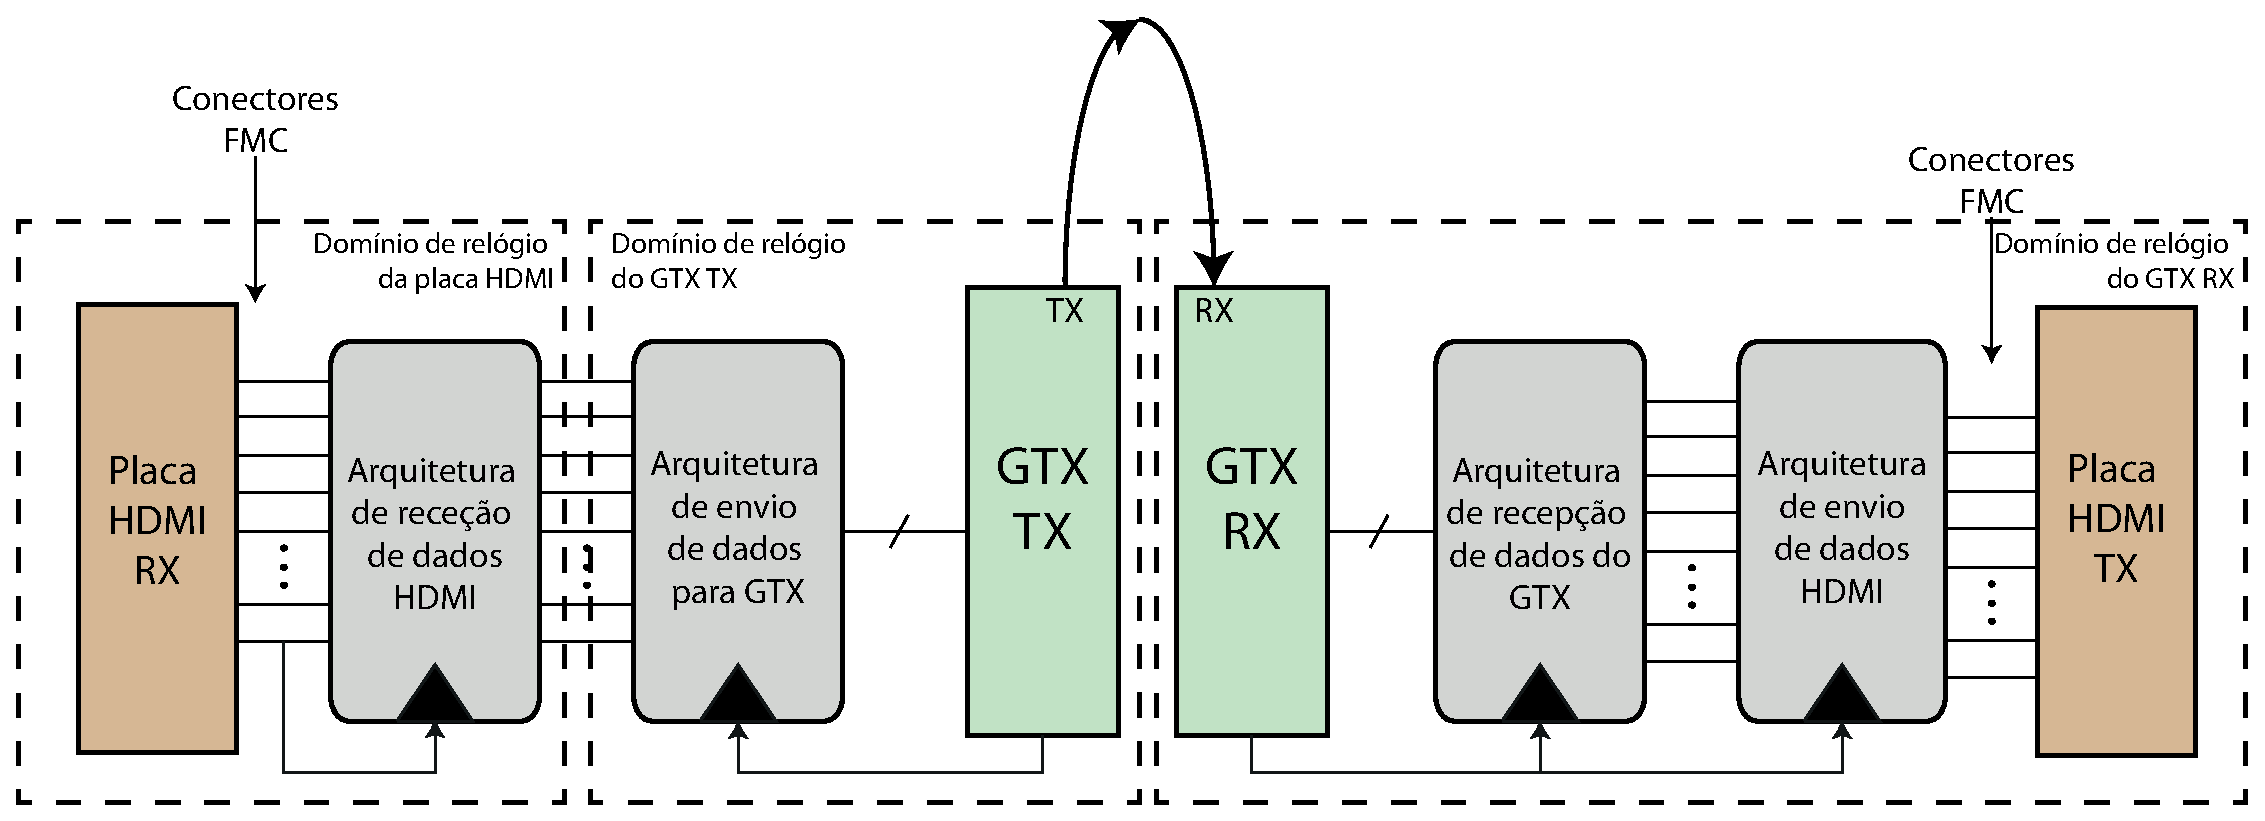
\includegraphics[width=1.0\textwidth]{diagrama_dominios} 
				\caption{Dominios de relógio nestas implementações}
				\label{fig:dominos}
			\end{center}
		\end{figure}
	
	\section{Material Utilizado}
	Para a implementação destas arquitetursa são utilizados vários equipamentos, entre os quais os seguintes:
	\subsection{FPGA VC7203}
	É uma FPGA (\textit{Field-programmable gate array}) que se caracteriza pelo seu elevado número de recursos e também pelas entradas em saídas de alta velocidade que possui, tal como indica \cite{R008}. É utilizada para implementação do código desenvolvido em Verilog para estas arquiteturas, para conexão à placa HDMI pelos conectores FMC (\textit{FPGA Mezzanine Card}) e ainda para a transmissão de dados em série através entradas e saída de alta velocidade disponíveis (GTX - \textit{Gigabit Transceiver}).
	\subsection{TB-FMCH-HDMI2-TX e TB-FMCH-HDMI2-RX}
	Estas placsa HDMI caracterizam-se pela capacidade de transmissão e receção de dados HDMI. Para esta implementação, a placa deve estar configurada por omissão cujos detalhes se encontram em \cite{R009}.
	
	\section{Arquitetura}
	
	\subsection{Geração do módulo GTX}	

	Quando se gera o módulo GTX através da interface disponibilizada pelo \textit{software} VIVADO existem algumas decisões que necessitam de ser tomadas para além das que já foram mencionados. Essas passam de seguida a ser detalhadas:
	
	Do lado do transmissor tomaram-se as seguintes principais decisões:
	\begin{enumerate}
		%	\item \textbf{\textit{Line Rate:}} Como referido anteriormente é 5,94 Gb/s.
		%	\item \textbf{Frequência de Amostragem das Tramas:} Assim como referido anteriormente é 148,5 MHz.
		%	\item \textbf{Tamanho da interface com a FPGA:} Tal como explicado em \ref{subsub:planD_considerações} na página \pageref{subsub:planD_considerações} é 40 bits
		\item \textbf{Tamanho interno dos dados:} Esta escolha envolve o número de caminhos de dados (\textit{datapath}) que são utilizados e ainda o valor da frequência de TXUSRCLK. Escolheu-se 40 bits para tal, o que implica o uso de apenas um \textit{datapath}, obtendo-se as frequências idênticas de TXUSRCLK e TXUSRCLK2.
		\item \textbf{Tipo de codificação:} Neste caso não se escolheu codificação porque não é possível (a interface com a FPGA é de 40 bits) e também numa fase inicial optou-se por simplificar o projeto.
		\item \textbf{Escolha ente \textit{Buffer} ou Bloco de Alinhamento de Fase:} Foi escolhido a utilização do \textit{buffer} uma vez que é de mais fácil utilização não requerendo o uso de lógica extra (comparativamente ao bloco de alinhamento de fase) e ainda assim é robusto.
	\end{enumerate}
	
	Do lado do recetor as principais decisões tomadas foram as seguintes:
	\begin{enumerate}
		\item \textbf{Tipo de equalização:} Apesar de este ser um projeto simples em que não se pretende inserir o sinal em canais ruidosos, optou-se por utilizar um equalizador DFE uma vez que traz mais vantagens do que a utilização do equalizador LPM.
		
		\item \textbf{Alinhamento de palavras:} Como palavra de alinhamento escolheu-se o símbolo K28.3 (mais informação pode ser encontrada em \cite{R041}). Contudo, é necessário ter em conta que não se está a utilizar codificação e, como tal, para efetuar o alinhamento da palavra o recetor não alinha pelo símbolo K28.3 codificado, mas sim, não codificado. Ou seja, na realidade quando encontrar a palavra ``7C'' assume que é a palavra de alinhamento e a trama passa a estar alinhada para esse limite. Para além disso, optou-se por ativar a porta ``RXSLIDE'' que ativa o alinhamento manual dos bits, pois é de esperar que seja necessário ativar o alinhamento manual para ligações cuja taxa de débito seja superior a \SI{5}{\giga\bit\per\second}.
		
		\item \textbf{Tipo de descodificação:} Não foi utilizada nenhuma descodificação, pois do lado do transmissor também não há codificação.
		\item \textbf{Escolha ente \textit{Buffer} ou Bloco de Alinhamento de Fase:} Optou-se pela escolha do \textit{buffer}, porque no caso do recetor para além não requerer lógica extra e ter uma inicialização mais rápida (comparativamente ao bloco de alinhamento de fase), também não exige que a correção do sinal de relógio seja realizada fora do transcetor, tal como indicado em \cite{R011}.
	\end{enumerate}
	
	\begin{table}[h!]
		\centering
		\caption[Sumário do módulo GTX gerado para a transmissão em série de uma barra de cores gerada na FPGA]{Sumário do módulo GTX gerado para a transmissão em série de uma barra de cores gerada na FPGA (adaptada do \textit{software})}
		\label{table:sumario_planoD}
		\begin{tabular}{@{}ll@{}}
			\toprule
			\multicolumn{1}{c}{\textbf{Característica}} & \multicolumn{1}{c}{\textbf{GT}} \\ \midrule
			\textbf{TX Line Rate (Gbit/s)}                & \num{5,94}                            \\
			\textbf{TX Reference Clock (MHz)}           & \num{148.5}                         \\
			\textbf{Enconding}                          & None                            \\
			\textbf{TX Internal Data Width}             & 40                              \\
			\textbf{TX External Data Width}             & 40                              \\
			\textbf{TXUSRCLK (MHz)}                     & 148,5                           \\
			\textbf{TXUSRCLK2 (MHz)}                    & 148,5                           \\
			\textbf{TX Buffer Enabled}                  & TRUE                            \\
			\textbf{RX Line Rate (Gbit/s)}                & \num{5,94}                            \\
			\textbf{RX Reference Clock (MHz)}           & \num{148.5}                           \\
			\textbf{Decoding}                           & None                            \\
			\textbf{RX Internal Data Width}             & 40                              \\
			\textbf{RX External Data Width}             & 40                              \\
			\textbf{RXUSRCLK (MHz)}                     & \num{148.5}                           \\
			\textbf{RXUSRCLK2 (MHz)}                    & \num{148.5}                           \\
			\textbf{RX Buffer Enabled}                  & TRUE                            \\ \bottomrule
		\end{tabular}
	\end{table}
	
	Na tabela \ref {table:sumario_planoD} é apresentada uma tabela sumário do módulo gerado. Esta tabela foi adaptada da interface que gera o módulo.

	\subsection{Arquitetura D} \label{sub_planD}
	Na figura \ref{fig:planoD} visualiza-se o diagrama de blocos desenvolvido para esta arquitetura com os seus diversos sub-módulos. 
	
		\begin{figure}[h!]
			\begin{center}
				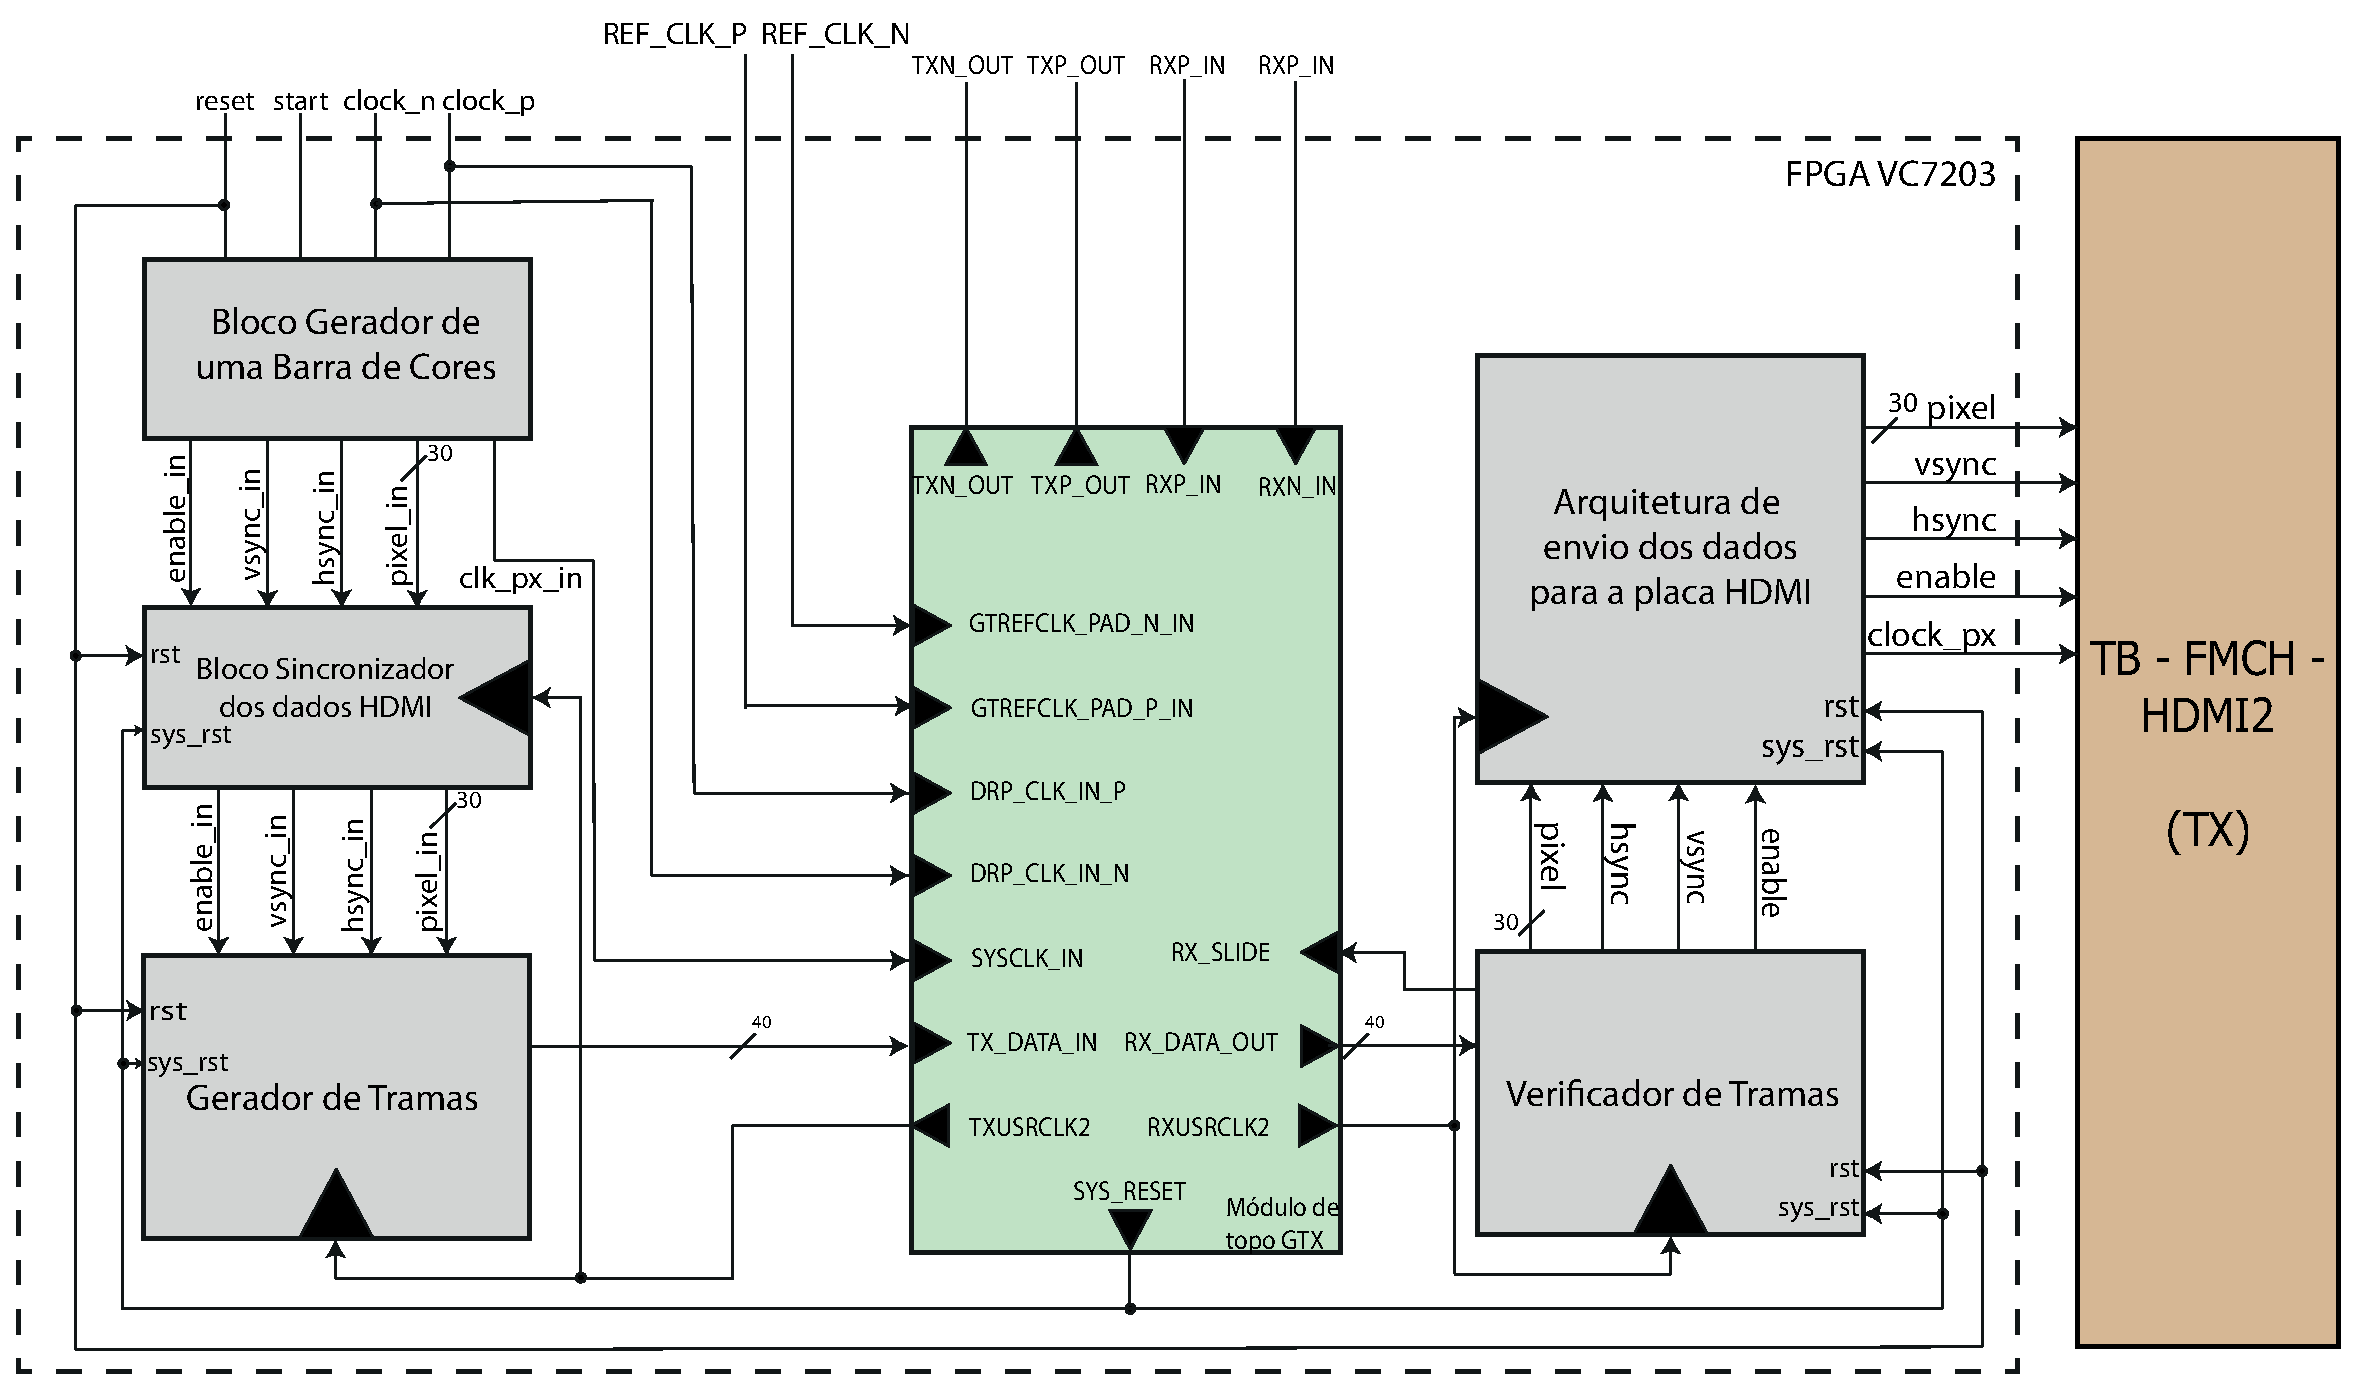
\includegraphics[width=1.0\textwidth]{planod} 
				\caption{Diagrama de blocos da arquitetura D}
				\label{fig:planoD}
			\end{center}
		\end{figure}
	
	\subsubsection*{Bloco gerador de uma Barra de Cores} \label{subsub:serial_colorBarGenerator}
	
	Este bloco gerador de barra de cores tem a seguinte funcionalidade: gera uma barra de cores em \textit{FULL HD} com uma frequência de \SI{148.5}{\mega\hertz}. Nas suas entradas encontram-se as portas vindas diretamente do exterior, tal como nas outras arquiteturas que utilizam este bloco. Estas são os botões definidos pelo utilizador (\textit{reset} e \textit{start}) e também um sinal de relógio diferencial de \SI{200}{\mega\hertz}. Nas suas saídas encontram-se os sinais referentes à imagem gerada que são posteriormente enviados para um bloco sincronizador dos dados HDMI.
	
	\subsubsection*{Bloco Sincronizador dos dados HDMI} \label{subsub:serial_syncsignals}
	
	O recurso a este bloco sincronizador dos dados HDMI deve-se aos diferentes domínios de relógio que existem no sistema: por um lado existe um bloco que gera uma barra de cores a uma determinada cadência, e por outro existe um bloco que gera as tramas a serem enviadas para o transcetor a outra cadência. Estes dois sinais de relógio podem ser iguais, no entanto podem não estar em fase o que é suficiente para haver problemas de meta-estabilidade. 
	
	Por este motivo, este bloco de sincronização é apenas constituído por dois registos de deslocamento (\textit{shift-registers}) para que problemas de sincronização que possam eventualmente existir sejam resolvidos. O diagrama de blocos deste módulo é apresentado na figura \ref{fig:sync_block}. 
	
	\begin{figure}[h!]
		\begin{center}
			\leavevmode
			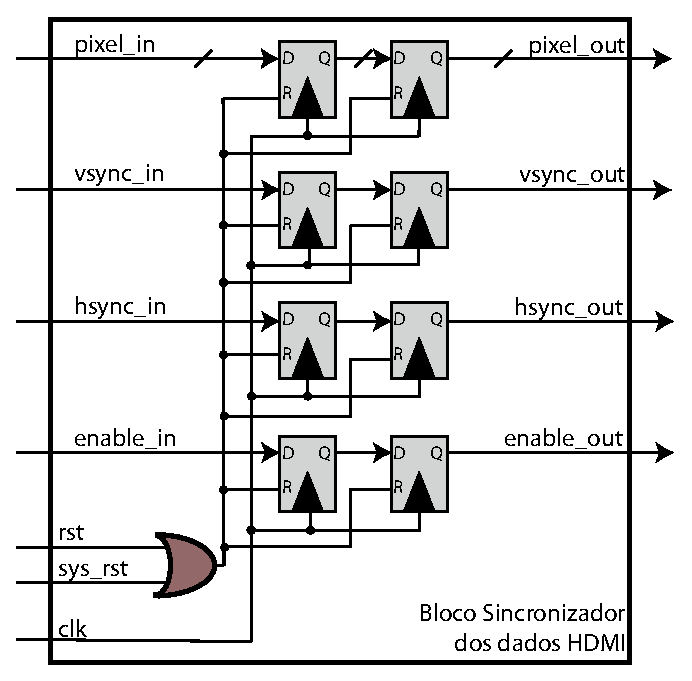
\includegraphics[width=0.5\textwidth]{sync_block_from_HDMI}
			\caption[Bloco de sincronização de dados]{Bloco de sincronização de dados}
			\label{fig:sync_block}
		\end{center}
	\end{figure}
	
	Tal como se visualiza na figura, para além de nas suas entradas se encontrar os dados provenientes da fonte HDMI há também dois sinais : \textit{rst} e \textit{sys\_rst}. O primeiro sinal refere-se ao sinal de \textit{reset} controlado pelo utilizador e o segundo corresponde a um sinal de \textit{reset} ativado automaticamente pelo módulo GTX.
	
	O sinal de relógio a que opera este bloco trata-se do sinal de relógio proveniente do módulo GTX, tal como se visualiza na figura \ref{fig:planoD}.
	
	\subsubsection*{Gerador de Tramas} \label{subsub:serial_frameGenerator}
	
	Este bloco é responsável pela criação das tramas a serem enviadas para o módulo GTX. Relembra-se que nesta abordagem inicial do projeto não se teve em conta a criação de tramas bem definidas para todos os momentos de transmissão. 
	
	Definiu-se a trama correspondente ao início da transmissão para que seja possível manter o alinhamento do lado do recetor e iniciar o processo. Esta é designada por  SOP (\textit{Start of Packet}) e é enviada em momentos de transmissão nulos, ou seja, quando os sinais de controlo da imagem se encontram inativos ($vsync = 0$, $hsync = 0$ e $enable = 0$), sendo constituída por 40 bits que em hexadecimal corresponde a: 000605047c. Este padrão sugerido pelo exemplo disponibilizado no \textit{software} da \textit{Xilinx} possui as seguintes particularidades:
	
	\begin{enumerate}
		\item No final da mesma encontra-se a palavra de alinhamento (conjunto dos primeiros bits a ser transmitido) que permite ao transcetor alinhar a trama internamente.
		\item Nunca será confundida como trama de informação (apresentada na figura \ref{fig:trama_abordagem_inicial}) devido à composição dos últimos 7  bits de ambas. A trama SOP termina em 1111100, e a trama de informação termina em 1010101.
	\end{enumerate}
	
	
	
	%%Explicar como são os pacotes noutras alturas de transmissão sem ser qdo se envia SOP
	Quando algum sinal de controlo referente à imagem está ativo é transmitida uma trama de informação com o formato que se visualiza na figura \ref{fig:trama_abordagem_inicial}.
	
	\begin{figure}[h!]
		\begin{center}
			\leavevmode
			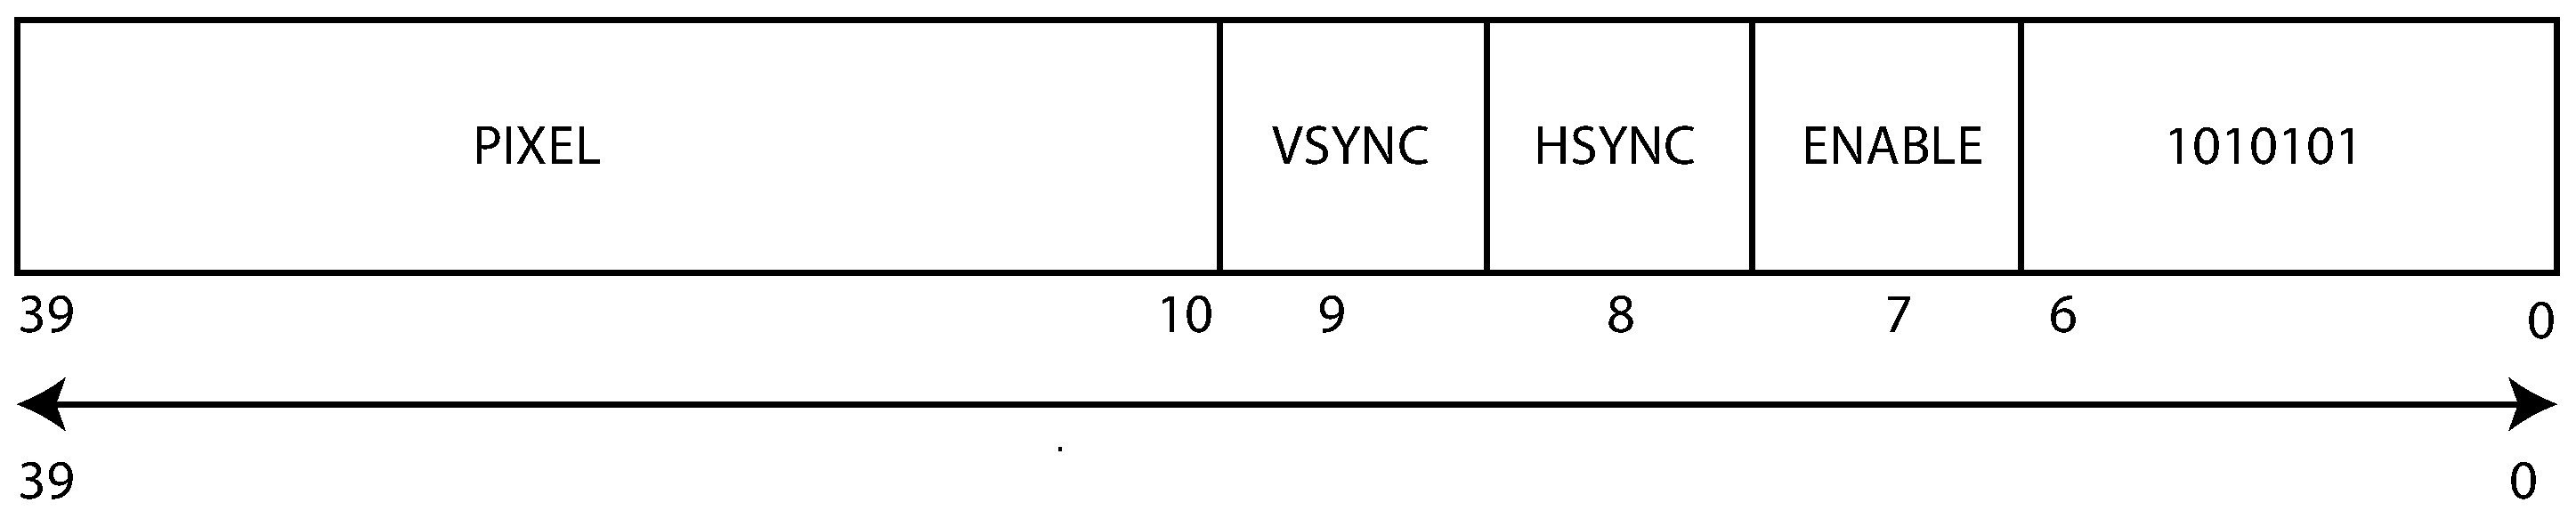
\includegraphics[width=1.0\textwidth]{trama_abordagem_inicial}
			\caption[Estrutura das tramas de informação]{Estrutura das tramas de informação}
			\label{fig:trama_abordagem_inicial}
		\end{center}
	\end{figure}
	
	Assim sendo, consoante os dados que recebe nas suas entradas (\textit{pixel}, \textit{vsync}, \textit{hsync} e \textit{enable}), este bloco ou envia SOP ou envia tramas de informação. A figura \ref{fig:momentos_tramas} exemplifica os diversos momentos de transmissão das diferentes tramas numa imagem. A cinza correspondem os momentos da imagem em que os sinais de controlo da mesma estão inativos, e por isso são transmitidas tramas SOP. A castanho correspondem os momentos de transmissão em que algum dos sinais de controlo de imagem está ativo e por isso são enviadas tramas de informação. Sempre que o sinal \textit{rst} ou \textit{sys\_rst} estiver ativo os dados são repostos e as tramas enviadas são SOP. 
	
	\begin{figure}[h!]
		\begin{center}
			\leavevmode
			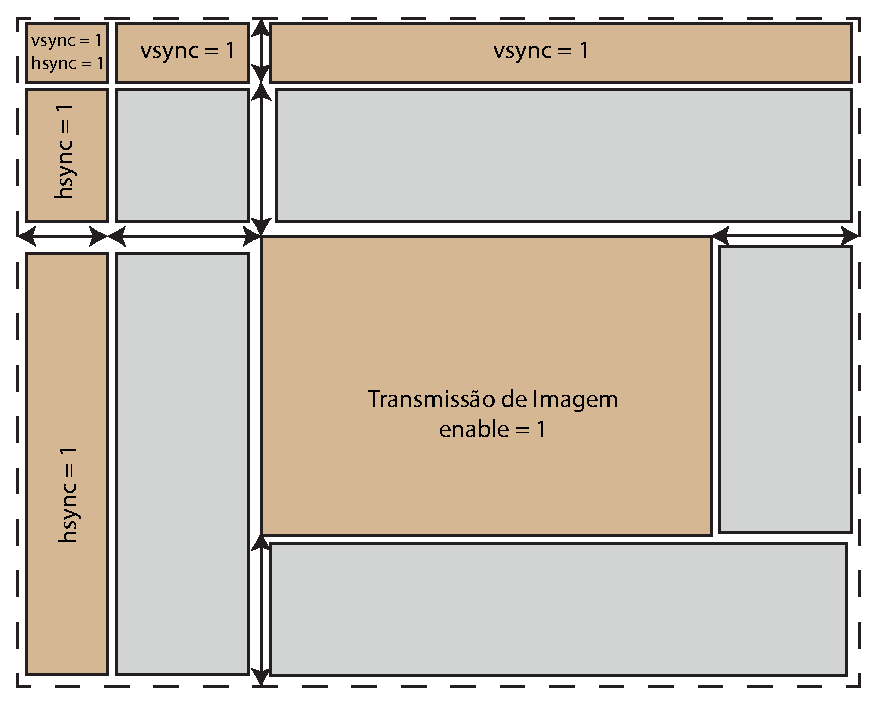
\includegraphics[width=1.0\textwidth]{exemplo_tramas_transmissoes}
			\caption[Momentos de transmissão de diferentes tramas]{Momentos de transmissão de diferentes tramas}
			\label{fig:momentos_tramas}
		\end{center}
	\end{figure}
	
	É de esperar que a transmissão demore algum tempo a alinhar do lado do recetor, sendo necessário que as tramas SOP sejam enviadas durante algum tempo. Por este motivo escolheram-se os momentos de transição de dados de controlo nulos, pois são suficientemente longos para que a transmissão possa ser alinhada. Assim, no pior dos casos, perde-se a primeira imagem completa que é transmitida, pois não são recebidos os primeiros dados de controlo (\textit{vsync} e \textit{hsync}) mas garante-se que todas as outras estão alinhadas e os dados serão corretamente recebidos do lado do transmissor.
	
	\subsubsection*{Verificador de Tramas} \label{subsub:serial_frameChecker}
	
	%%Explicar porque existe
	
	Este bloco é responsável pela re-organização das tramas recebidas que são recebidas à cadência RXUSRCLK2. Apesar de poder parecer que com o alinhamento interno as tramas chegariam ao recetor tal como são enviadas do transmissor, isso raramente se verifica. As tramas são alinhadas para um determinado limite assim que o recetor encontra a palavra de alinhamento. %, no entanto não significa que a trama recebida é exatamente igual à trama enviada. 
	
	Segundo \cite{R022} e \cite{R011}, quando a palavra de alinhamento é detetada no recetor, este assume que os dados a partir daí são válidos e alinha-os para um determinado limite. Este limite pode ser selecionado aquando a criação do módulo GTX, tendo-se optado por alinhar os dados para o \textit{byte} mais próximo. Apesar de não se estar a lidar com codificação e devido ao tamanho do \textit{datapath} ser 40 bits, o bloco de alinhamento das palavras considera que 1 \textit{byte} são 10 bits (a codificação 8B/10B codifica 8 bits em 10 bits). Assim, quando é detetada a palavra de alinhamento as tramas recebidas no recetor podem chegar de quatro maneiras diferentes ilustradas na figura \ref{fig:alinhamento_tramas_gtx}.
	
	
	%Se o datapath fosse de 32 bits sem codificação, assumiria que 1 \textit{byte} sao 8 bits, de certeza, apesar de eu nao ter testado
	\begin{figure}[h!]
		\begin{center}
			\leavevmode
			\includegraphics[width=1.0\textwidth]{organizacao_tramas}
			\caption[Alinhamento das tramas no transcetor]{Alinhamento das tramas no transcetor}
			\label{fig:alinhamento_tramas_gtx}
		\end{center}
	\end{figure}
	
	Daí a importância da trama de SOP: quando é detetada em algum dos limites assinalados a cinzento dá-se início à transmissão dos restantes dados. Para se proceder à organização dos dados recebidos é necessário recorrer a uma máquina de estados. Esta foi adaptada da que a ferramenta de \textit{software} cria por omissão quando é gerado um exemplo deste módulo GTX.
	
	A máquina de estados principal é dividida em três por questões de simplificação e de melhor entendimento da mesma. Cada uma destas divisões passa a ser detalhada, sem nunca esquecer que funcionam como um todo.
	%%Explicar máquina de estados que procura dados, ou espera ou tal e tal
	
	\begin{enumerate}
		\item \textbf{Máquina de estados geral da receção de dados:}
		
		Esta máquina é composta por três estados que definem o estado geral da receção de dados. Estes estados são:
		\begin{itemize}
			\item \textbf{\textit{Begin:}} Estado inicial que aguarda a receção de dados válidos do recetor. Quando a trama de SOP é detetada pela primeira vez, então a máquina transita para um estado em que recebe dados válidos. 
			
			\item \textbf{\textit{Track\_data:}} Neste estado já foi detetato o início da transmissão (SOP) e por isso todos os dados que estão a ser recebidos são considerados válidos. Quando é detetado algum erro (com a ajuda de uma máquina de estados detetora de erros) transita de estado.
			
			\item \textbf{\textit{Data\_error\_detected:} }Estado de deteção de erro que transita imediatamente para o estado inicial para aguardar a chegada de dados válidos novamente.
			
		\end{itemize}
		
		Sempre que for necessário fazer \textit{reset} ao sistema, quer pela ativação do utilizador ou então pelo transcetor, volta-se ao estado inicial ``\textit{begin}''.
		
		
		\begin{figure}[h!]
			\begin{center}
				\leavevmode
				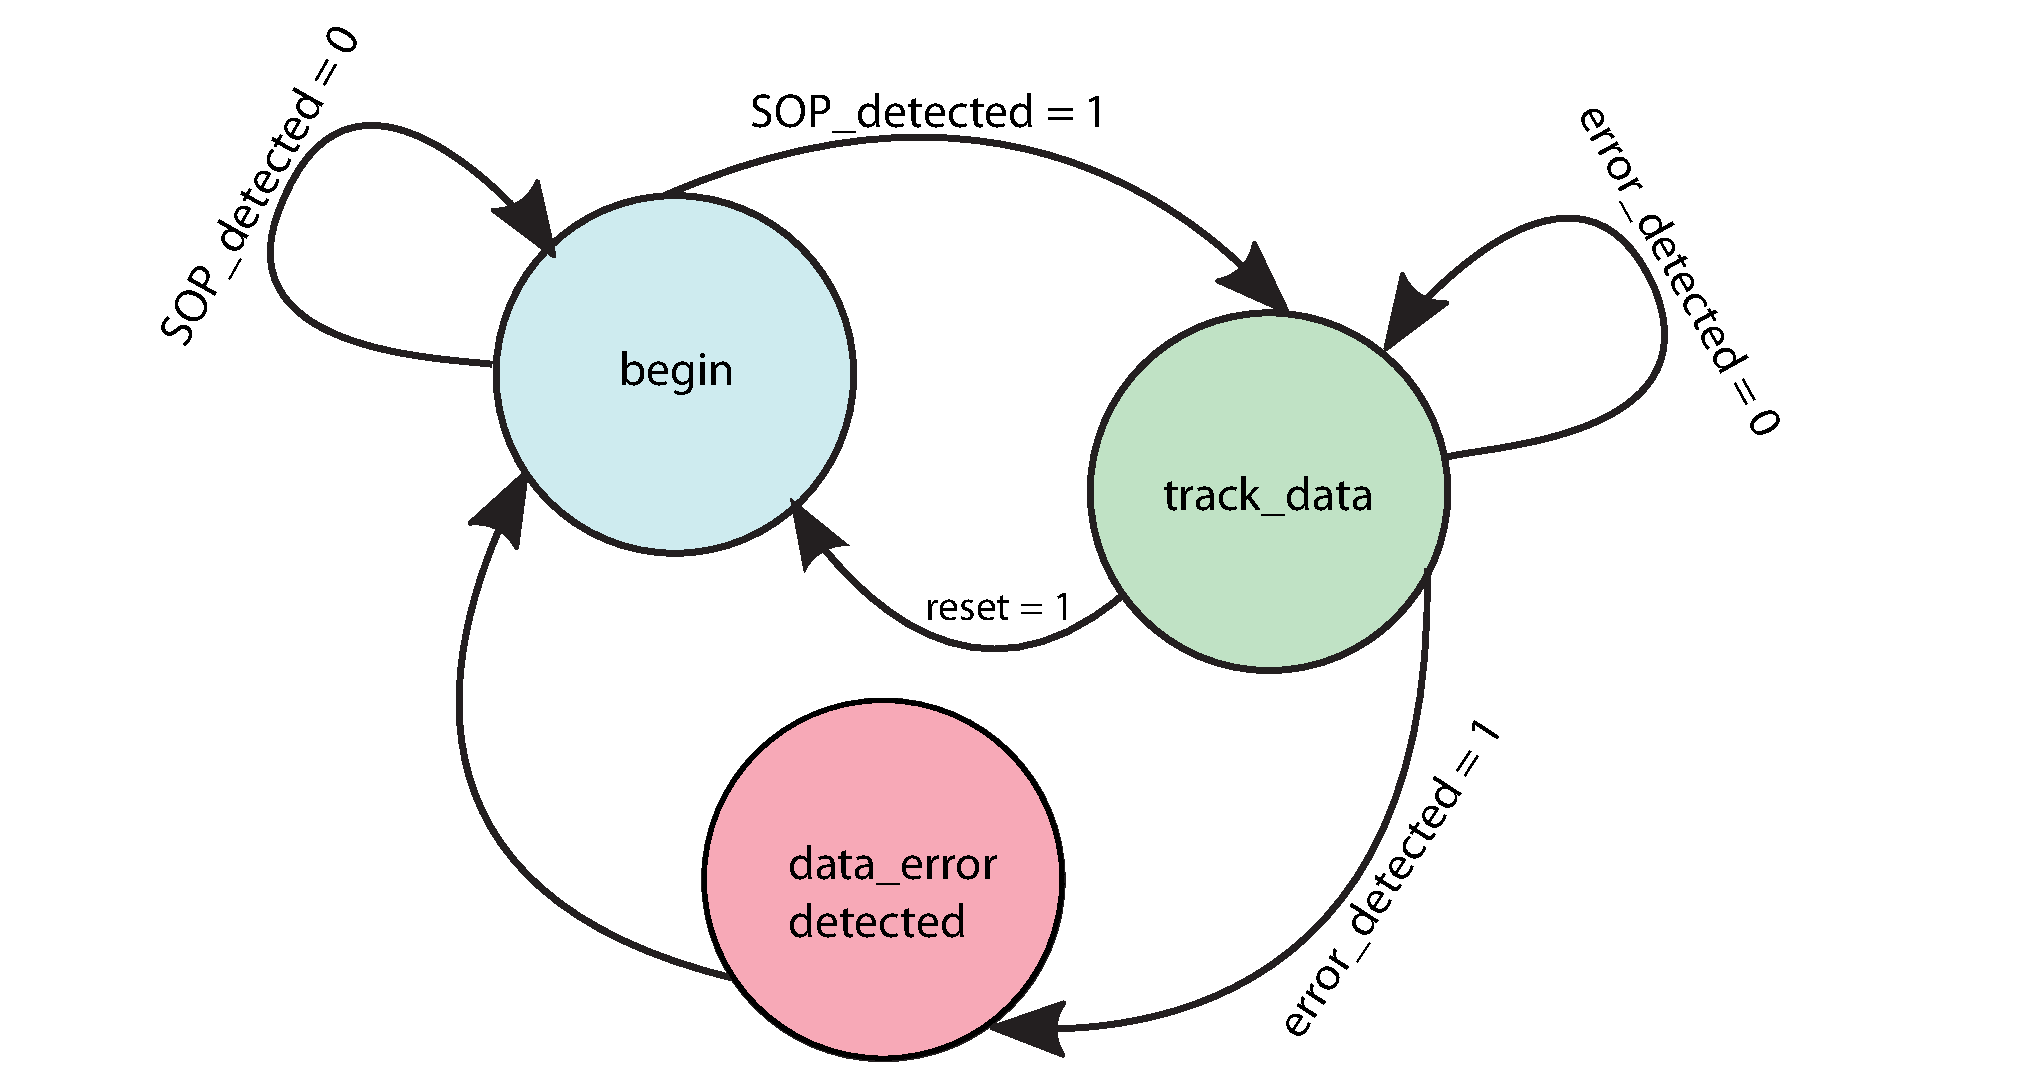
\includegraphics[width=1.0\textwidth]{fsm1}
				\caption[Máquina de estados de transmissão]{Máquina de estados de transmissão}
				\label{fig:FSM1}
			\end{center}
		\end{figure}
		
		A figura \ref{fig:FSM1} representa a máquina de estados detalhada anteriormente. De notar que na imagem estão representadas algumas \textit{flags} de decisão de transição de estados. A \textit{flag} ``\textit{SOP\_detected}'' indica que se a trama de início de pacote foi encontrada nos dados recebidos e ``\textit{error\_detected}'' indica que foi detetado um erro nos dados recebidos. Ambas são definidas por máquinas de estados que serão explicadas mais adiante.
		
		
		\item \textbf{Máquina de leitura de dados}
		
		Esta máquina de estados é responsável pela constante procura de dados recebidos pelo recetor. Destes apenas são guardadas as últimas duas tramas porque da sua combinação resulta a indicação de início de transmissão, iniciando o funcionamento desta máquina de estados.
		
		A figura \ref{fig:fsm2} ilustra a máquina de estados aqui referida, contudo antes de se detalhar os diferentes estados da mesma, faz-se uma breve descrição das \textit{flags} de transição de estados presentes na figura:
		
		\begin{figure}[h!]
			\begin{center}
				\leavevmode
				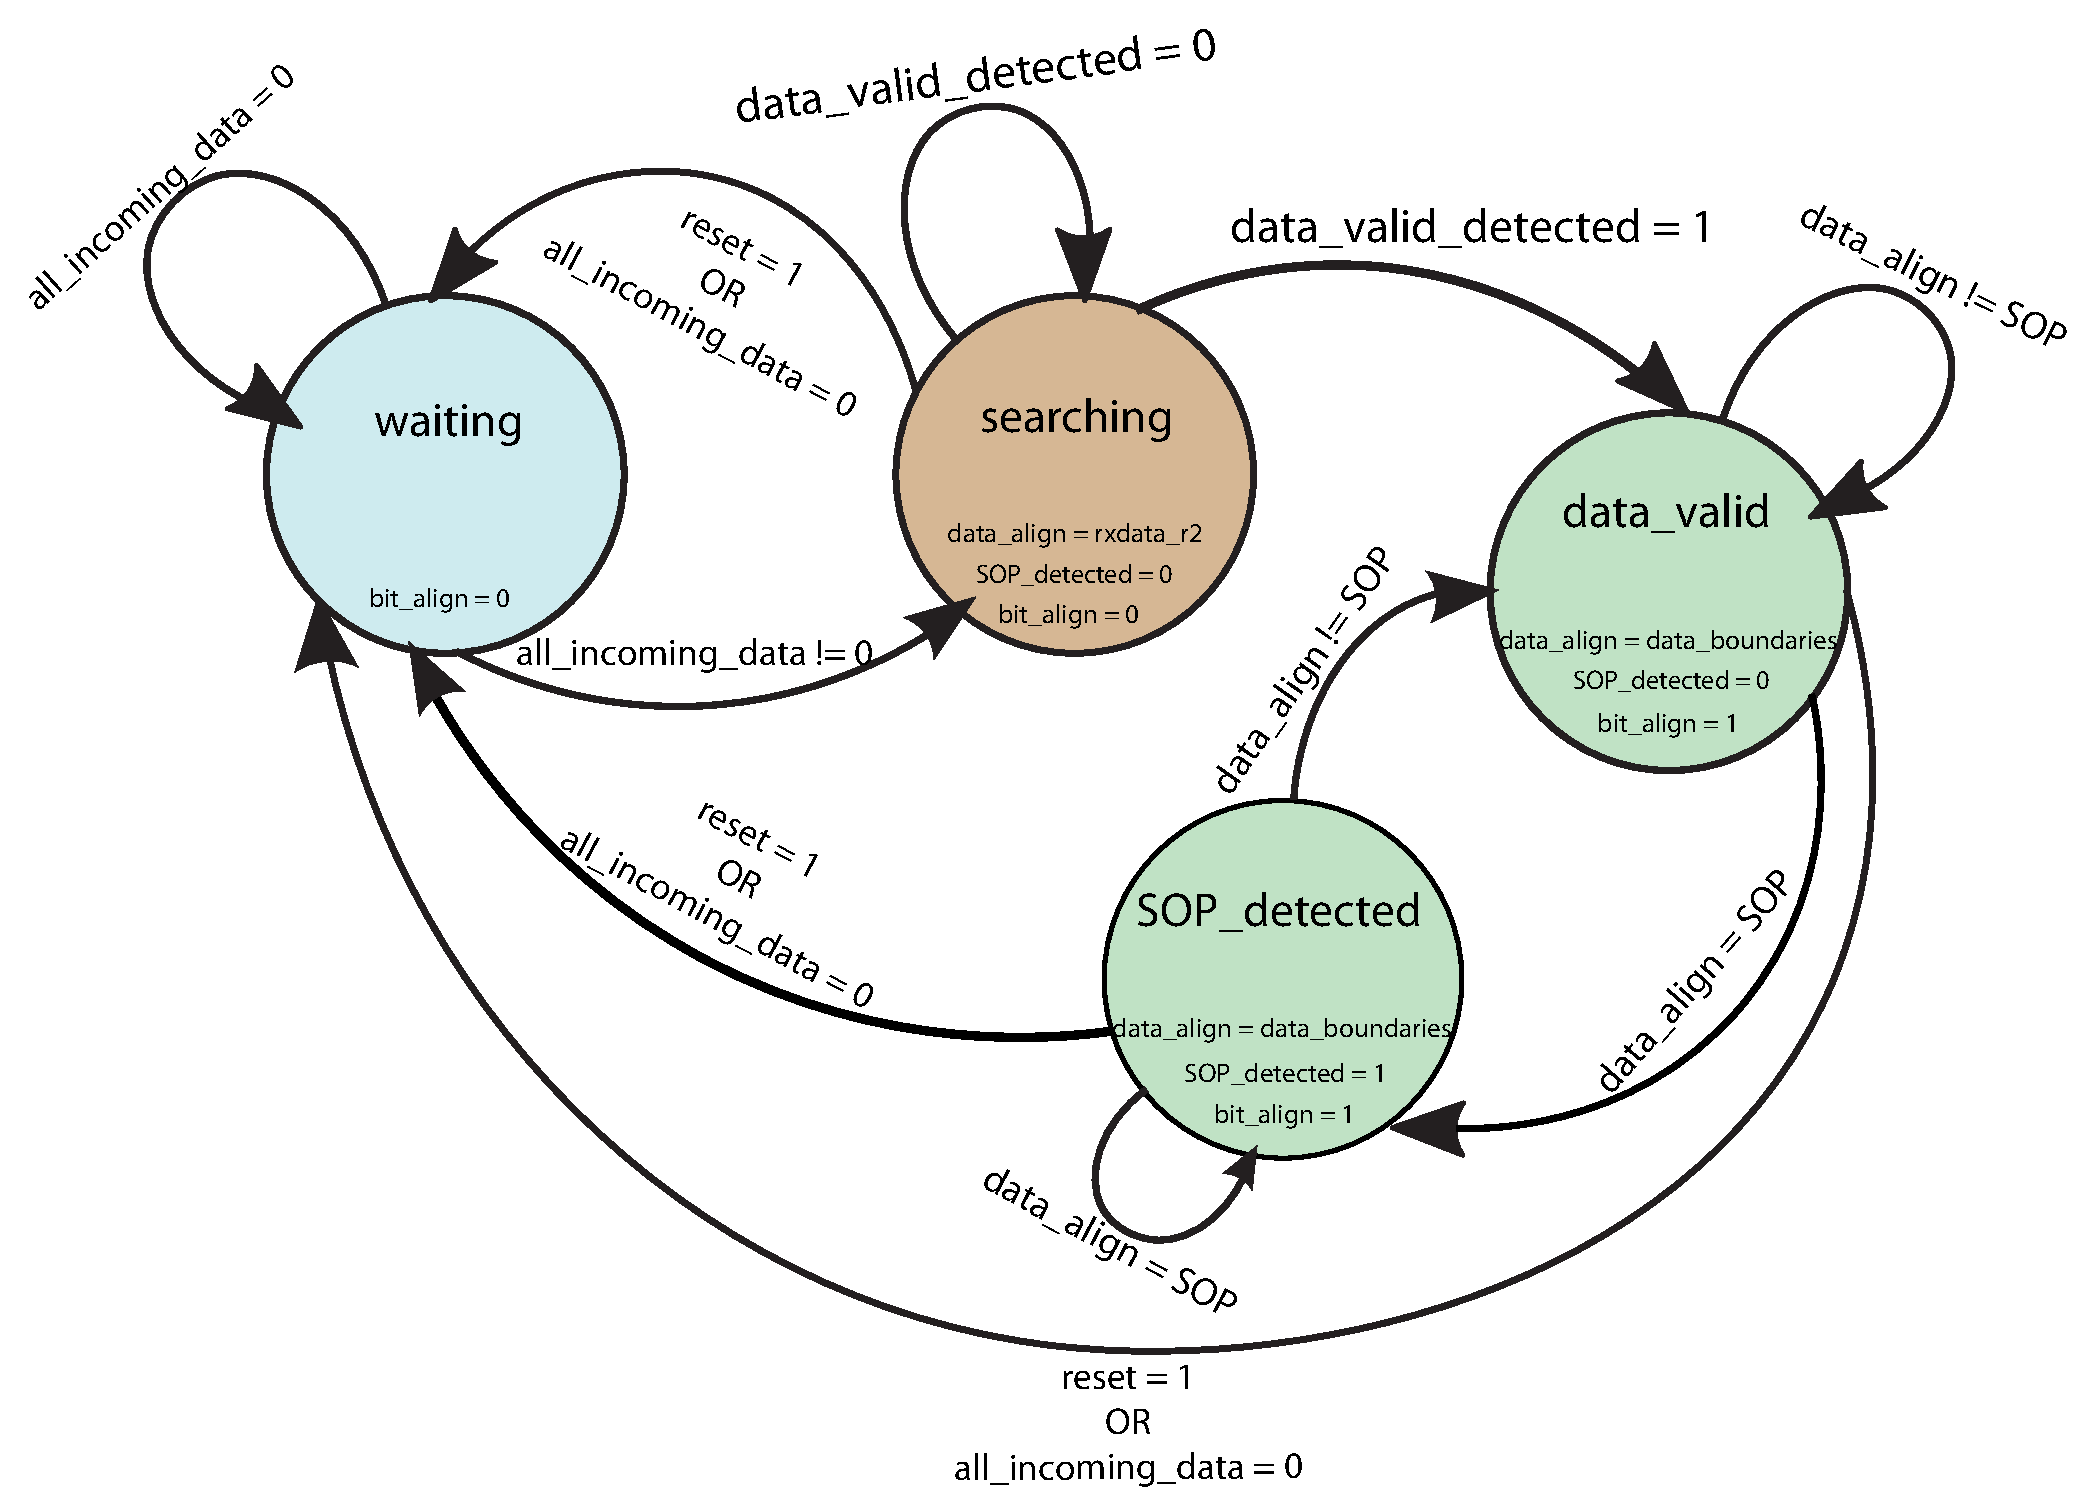
\includegraphics[width=1.0\textwidth]{fsm_track_data}
				\caption[Máquina de estados leitura de dados]{Máquina de estados leitura de dados}
				\label{fig:fsm2}
			\end{center}
		\end{figure}
		
		\begin{itemize}
			\item \textit{all\_incoming\_data}: Esta \textit{flag} indica se todos os bits presentes nas duas últimas tramas recebidas no recetor são 0 ou não. Se sim, então a \textit{flag} é igual zero, senão é um.
			
			\item \textit{data\_valid\_detected}: Esta \textit{flag} indica se foi encontrado nos dados recebidos (nas duas últimas tramas) a trama SOP em alguma das situações assinaladas a cinza presentes na figura \ref{fig:alinhamento_tramas_gtx}.
			
			\item \textit{reset}: indica se foi ativado o sinal para repôr os dados originais da máquina de estados.
		\end{itemize}	 
		
		Estas são as principais \textit{flags} de transição de estados da máquina. De seguida serão detalhados todos os estados da mesma:
		
		\begin{itemize}
			\item \textbf{\textit{Waiting}:} Este estado indica que o recetor ainda não está a receber dados, isto porque a \textit{flag} \textit{all\_incoming\_data} está inativa. Por defeito, quando não há transmissão de dados do lado do transmissor, o recetor recebe apenas dados iguais a zero. Assim que esta \textit{flag} se ativa então passa-se para o estado \textit{searching}.
			
			\item \textbf{\textit{Searching}:} Neste estado, a máquina procura a trama que dá inicio à transmissão de dados (SOP). Uma vez que ela pode vir alinhada em diferentes \textit{bytes} nas tramas do recetor, então a máquina procura a SOP nas quatro situações apresentadas na figura \ref{fig:alinhamento_tramas_gtx}. Assim que encontra SOP, memoriza os limites das tramas em que esta foi encontrada para que se possa retirar todos os outros dados de transmissão e transita de estado.
			
			\item \textbf{\textit{Data\_valid}:} Este estado serve essencialmente para guardar os dados devidamente alinhados segundo os limites da trama SOP. Ativa-se a flag \textit{bit\_align} para que o sistema reconheça que os dados se encontram alinhados. Se os dados que estão a ser guardados em \textit{data\_align} corresponderem à trama SOP então transita-se de estado para indicar que esta trama foi detetada. 
			
			\item \textbf{\textit{SOP\_detected}:} Quando este estado está ativo, então os dados alinhados correspondem à trama SOP, e por isso deve-se ativar a \textit{flag} ``\textit{SOP\_detected}''. Este estado mantém-se ativo enquanto os dados alinhados corresponderem à trama SOP e transita para o estado ``\textit{data\_valid}'' assim que tal deixar de ser verdade. 
		\end{itemize}
		
		Sempre que a transmissão for interrompida (\textit{all\_incoming\_data} se iguala a zero) ou o sinal de \textit{reset} for ativo (quer por opção do utilizador ou pelo módulo GTX), então a máquina retorna ao estado inicial e repõe os dados originais do sistema. 
		
		Inicialmente o estado ativo é ``\textit{waiting}'', e todas as \textit{flags} de decisão de mudança de estado (\textit{all\_incoming\_data} e \textit{data\_valid\_detected}) estão igualadas a zero.
		
		
		\item \textbf{Máquina de estados de verificação do alinhamento dos dados}
		
		Tal como já foi mencionado anteriormente, para taxas de transmissão superiores a \SI{5}{\giga\bit\per\second} , o transcetor pode alinhar falsamente os dados. Por esse motivo, as tramas recebidas podem não vir dentro dos limites apresentados na figura \ref{fig:alinhamento_tramas_gtx}, sendo assim necessário o recurso a uma máquina de estados que valide o correto alinhamento.
		
		A máquina de estados apresentada na figura \ref{fig:fsm3} é responsável pela deteção do devido alinhamento das tramas recebidas de acordo com a figura \ref{fig:alinhamento_tramas_gtx}. Caso tal não se verifique procede ao alinhamento manual das tramas.
		
		\begin{figure}[h!]
			\begin{center}
				\leavevmode
				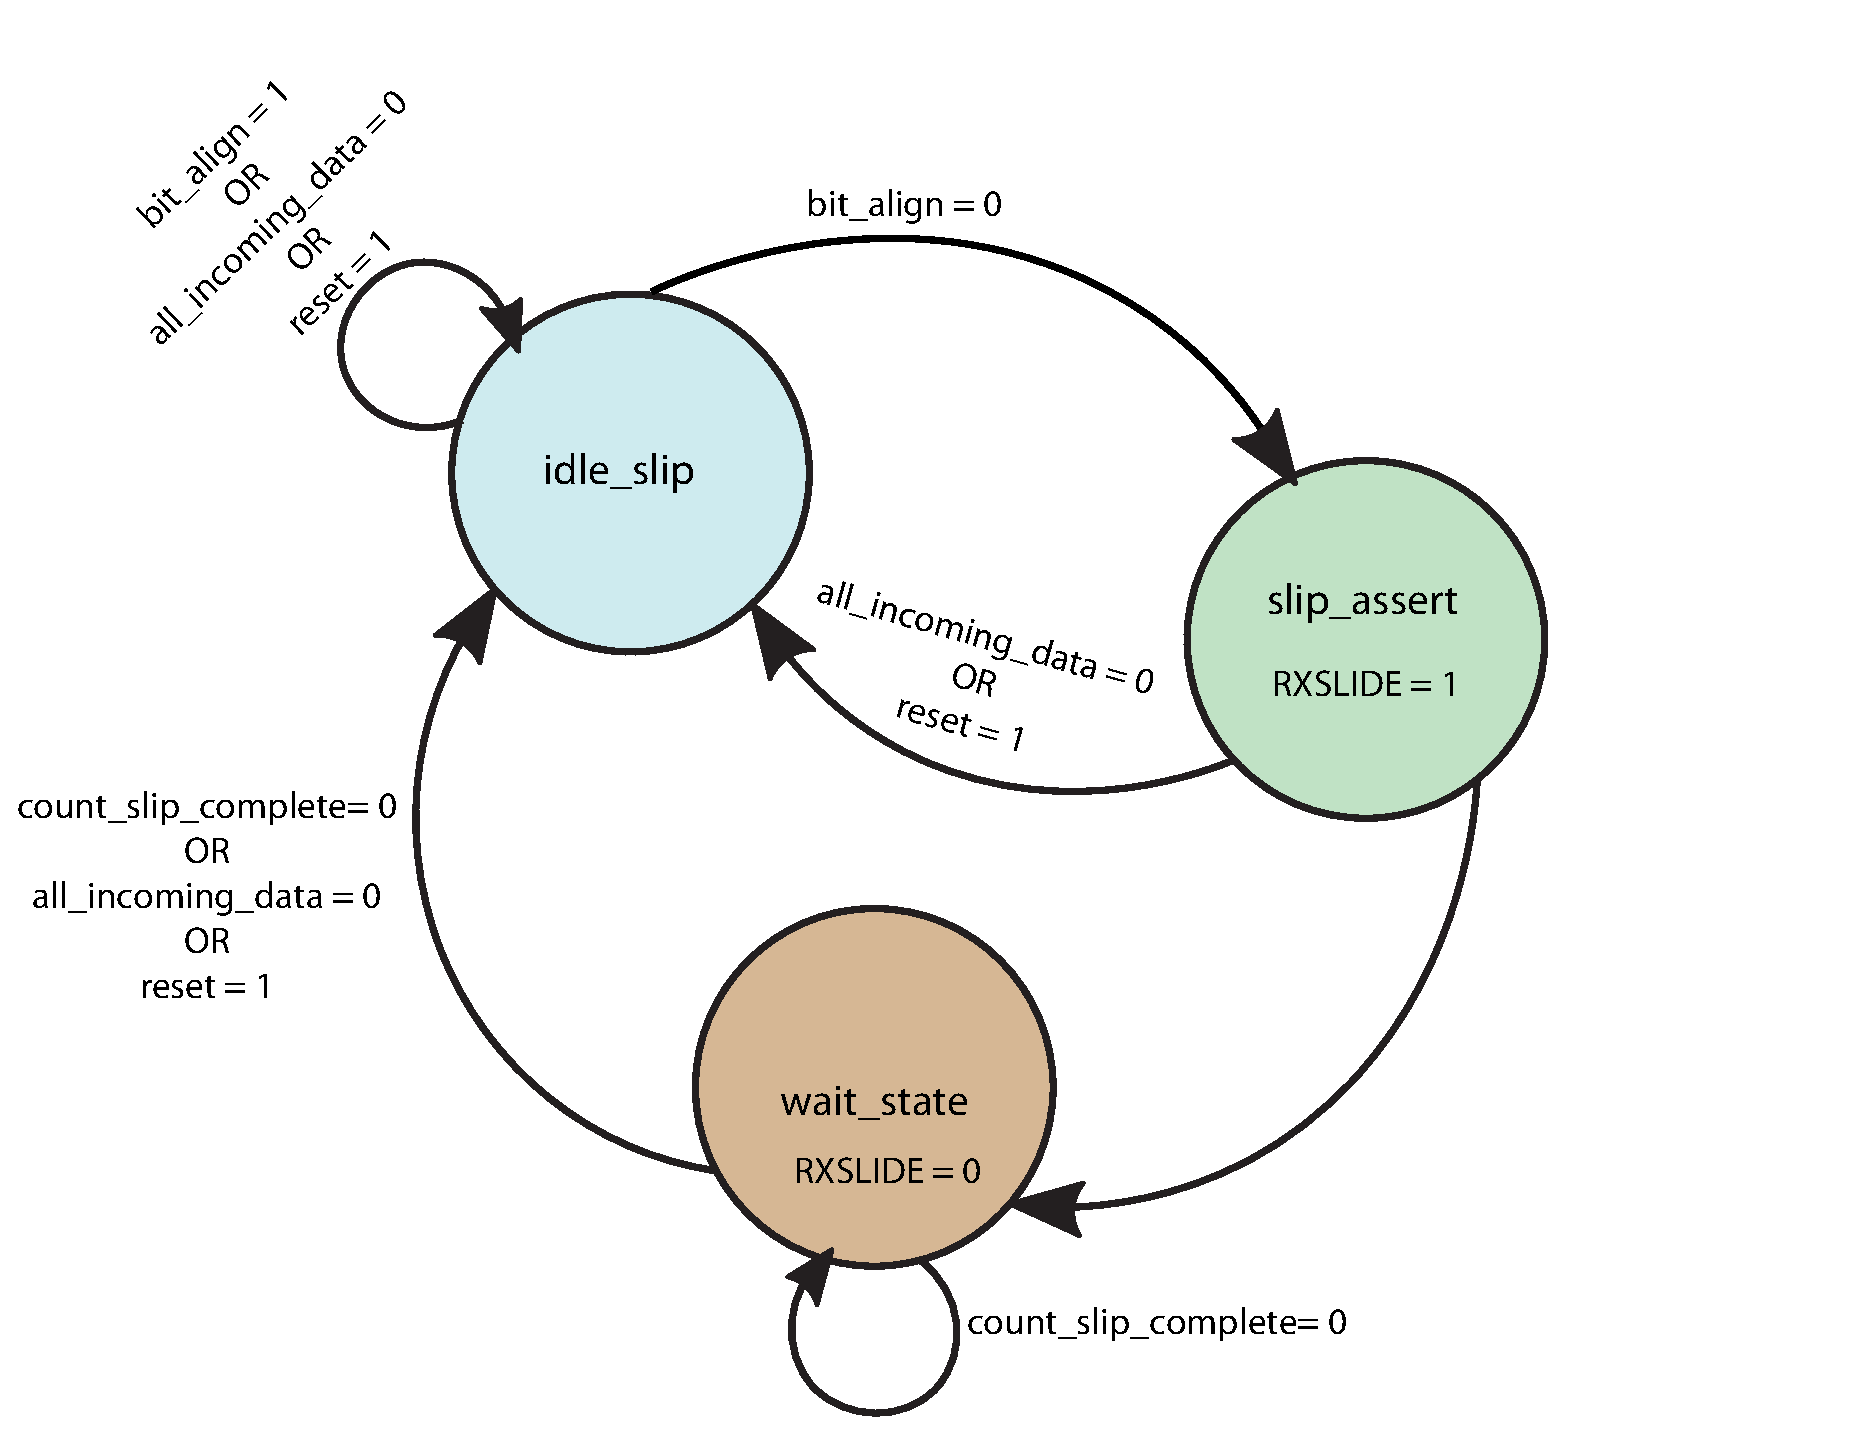
\includegraphics[width=1.0\textwidth]{fsm_bit_align}
				\caption[Máquina de estados de verificação do alinhamento dos dados]{Máquina de estados de verificação do alinhamento dos dados}
				\label{fig:fsm3}
			\end{center}
		\end{figure}
		
		%Descrição das flags
		Antes de se passar à descrição de cada estado, é de notar que existem algumas \textit{flags} de decisão de transição de estados:
		\begin{itemize}
			\item \textit{bit\_align}: Esta \textit{flag} indica se a palavra se encontra devidamente alinhada, tal como ilustrada na figura \ref{fig:alinhamento_tramas_gtx}. 
			
			\item \textit{all\_incoming\_data}: Esta \textit{flag} já foi mencionada e detalhada na máquina de estado que faz a leitura de dados.
			
			\item \textit{count\_slip\_complete}: Esta é uma \textit{flag} que fica ativa quando um contador termina (será explicado mais à frente).
			
			\item \textit{reset}: Indica a reposição dos dados originais da máquina de estados quando ativa.
		\end{itemize}
		
		%Descrição dos estados
		
		Esta máquina é composta por três estados, sendo estes:
		\begin{itemize}
			\item \textbf{\textit{Idle\_slip}:} Este estado aguarda pela receção de dados e também pela deteção do desalinhamento da palavra. Há transição de estado quando se verifica que as tramas que chegam ao recetor não estão alinhadas de acordo com os limites que deveriam estar.
			
			\item \textbf{\textit{Slip\_assert}:} Este estado está ativo quando há deteção de falso alinhamento de palavras, e por isso a saída que se conecta ao GTX é ativada: RXSLIDE. A ativação deste sinal vai permitir que as tramas sejam deslocadas em 1 bit. Este estado transita imediatamente para o estado de \textit{Wait\_state}.
			
			\item \textbf{\textit{Wait\_state}:} Neste estado o sinal de saída RXSLIDE volta a estar inativo e aguarda-se que a operação de deslocamento de 1 bit se verifique. Como estamos perante um \textit{datapath} de 40 bits, segundo \cite{R011} aguarda-se 64 ciclos de relógio. Após esta espera, a flag \textit{count\_slip\_complete} fica ativa e há transição de estado.
		\end{itemize}
		
		De notar que sempre que houver falha de transmissão ou o sinal de \textit{reset} for ativo, os sinais são repostos para os originais e volta-se ao estado \textit{Idle\_slip}.
		
		%Descrição dos dados originais da maquina
		
		Inicialmente o estado ativo é o {\textit{Idle\_slip} }e as \textit{flags} de sinalização de transição de estado são igualadas a 0.
		
		%	\item \textbf{Máquina que deteta os erros }
		%	\item \textbf{Máquina que deteta o estado da ligação}
	\end{enumerate}
	
	Para além destas máquinas de estados apresentadas existe a possibilidade de implementação de uma outra que verifique os erros das tramas recebidas. Esta máquina torna-se útil quando há implementação de códigos detetores de erros nas tramas, ativando a \textit{flag} ``\textit{error\_detected}'', sempre que o \textit{checksum} recebido na trama não corresponder à mensagem. Contudo, nesta abordagem inicial tal não é realizado e por isso essa \textit{flag} é globalmente igualada a zero.
	
	Quando os dados estão alinhados procede-se à extração da informação contida na trama recebida, enviando-a para o bloco responsável pela sua transmissão para a placa HDMI, sendo necessário que o estado  \textit{track\_data} esteja ativo. A informação retirada depende do tipo de trama recebida: caso a trama seja SOP, os dados são todos igualados a 0; caso contrário, então extrai-se os dados de acordo com o formato da trama de informação apresentado na figura \ref{fig:trama_abordagem_inicial}.
	
	
	%Se a trama recebida é uma SOP, igualam-se todos os dados a zero. Caso 
	%
	%Quando se recebe uma trama que é igual a SOP iguala-se todos os sinais a zero, no entanto quando a ligação está a procura de dados (o estado \textit{track\_data} está ativo) os dados são extraídos segundo o formato da trama enviada , representada na imagem  na página \pageref{fig:trama_abordagem_inicial}.
	
	\subsubsection*{Bloco de envio de dados para a placa HDMI} \label{subsub:serial_send signals to HDMI}
	
	Este bloco é responsável pela receção dos dados alinhados provenientes do bloco verificador de tramas e do seu posterior envio para a placa HDMI transmissora. A figura \ref{fig:sync_block_to_HDMI} é apresentado o diagrama de blocos deste módulo.
	
	\begin{figure}[h!]
		\begin{center}
			\leavevmode
			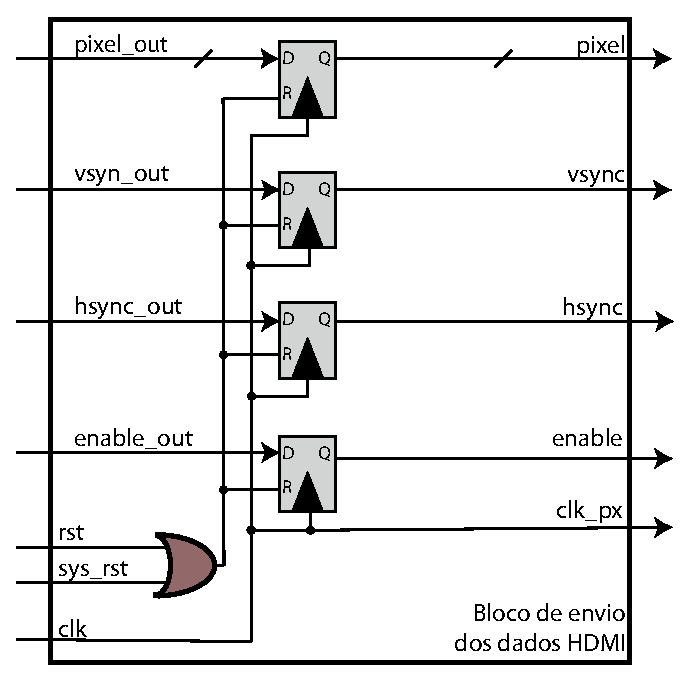
\includegraphics[width=0.5\textwidth]{sync_block_to_HDMI}
			\caption[Diagrama de blocos de envio de dados para a placa HDMI transmissora]{Diagrama de blocos de envio de dados para a placa HDMI transmissora}
			\label{fig:sync_block_to_HDMI}
		\end{center}
	\end{figure}
	
	Os dados recebidos neste bloco são lidos para um registo ao flanco positivo do sinal de relógio que alimenta este módulo (RXUSRCLK2). Posteriormente, todos os dados presentes nos registos são enviados para a placa HDMI transmissora incluindo o sinal de relógio RXUSRCLK2.
	
	\subsubsection*{Localizações das portas de saída do módulo de topo} \label{subsub:serial_locs_planD}
	
	Verifica-se que este bloco tem diversas entradas e saídas, e por isso para além de todo o código desenvolvido em Verilog para estes sub-módulo é necessário definir as localizações físicas da FPGA para cada porta de entrada e saída, estando as mesmas detalhadas na  tabela \ref{table:loc_planD_simples}. 
	
	%%%falar das portas todas
	\begin{table}[h!]
		\centering
		\caption[Localizações físicas das portas de entrada e saída da arquitetura desenvolvida]{Localizações físicas das portas de entrada e saída da arquitetura desenvolvida}
		\label{table:loc_planD_simples}
		%\resizebox{\textwidth}{!}{%
		\begin{tabular}{rlll}
			\hline
			\multicolumn{1}{l}{}                  & \multicolumn{1}{c}{\textbf{Sinal}} & \multicolumn{1}{c}{\textbf{LOC na FPGA}} & \multicolumn{1}{c}{\textbf{Banco na FPGA}} \\ \hline
			\multicolumn{1}{r|}{\textbf{Entrada}} & clk\_p                             & E19                                      & 38                                         \\
			\multicolumn{1}{r|}{\textbf{Entrada}} & clk\_n                             & E18                                      & 38                                         \\
			\multicolumn{1}{r|}{\textbf{Entrada}} & reset                              & N41                                      & 19                                         \\
			\multicolumn{1}{r|}{\textbf{Entrada}} & start                              & E42                                      & 19                                         \\
			\multicolumn{1}{r|}{\textbf{Entrada}} & REF\_CLK\_P                        & AF8                                      & 114                                        \\
			\multicolumn{1}{r|}{\textbf{Entrada}} & REF\_CLK\_N                        & AF7                                      & 114                                        \\
			\multicolumn{1}{r|}{\textbf{Entrada}} & RXP\_IN                            & AG6                                      & 114                                        \\
			\multicolumn{1}{r|}{\textbf{Entrada}} & RXN\_IN                            & AG5                                      & 114                                        \\
			\multicolumn{1}{r|}{\textbf{Saída}}   & TXN\_OUT                           & AK3                                      & 114                                        \\
			\multicolumn{1}{r|}{\textbf{Saída}}   & TXP\_OUT                           & AK4                                      & 114                                        \\
			\multicolumn{1}{r|}{\textbf{Saída}}   & clk\_px                            & E34                                      & 35                                         \\
			\multicolumn{1}{r|}{\textbf{Saída}}   & enable                             & K35                                      & 34                                         \\
			\multicolumn{1}{r|}{\textbf{Saída}}   & hsync                              & M32                                      & 34                                         \\
			\multicolumn{1}{r|}{\textbf{Saída}}   & vsync                              & L31                                      & 34                                         \\
			\multicolumn{1}{r|}{\textbf{Saída}}   & pixel{[}0{]} a pixel {[}29{]}      & Ver \cite{R041}                                & 34 e 35                                    \\ \hline
		\end{tabular}%
		%	}
	\end{table}
	
	
	\subsection{Arquitetura E}
		A figura \ref{fig:planoE} representa o digrama de blocos da arquitetura E. Através da visualização deste diagrama é possível concluir que o único sub-módulo adicionado é o bloco recetor de dados HDMI. Todos os outros sub-módulos são exatamente iguais ao da arquitetura anterior, estando detalhados na subsecção \ref{sub_planD}. Assim sendo, apenas será apresentado nesta subsecção esse mesmo bloco.
		\begin{figure}[h!]
			\begin{center}
			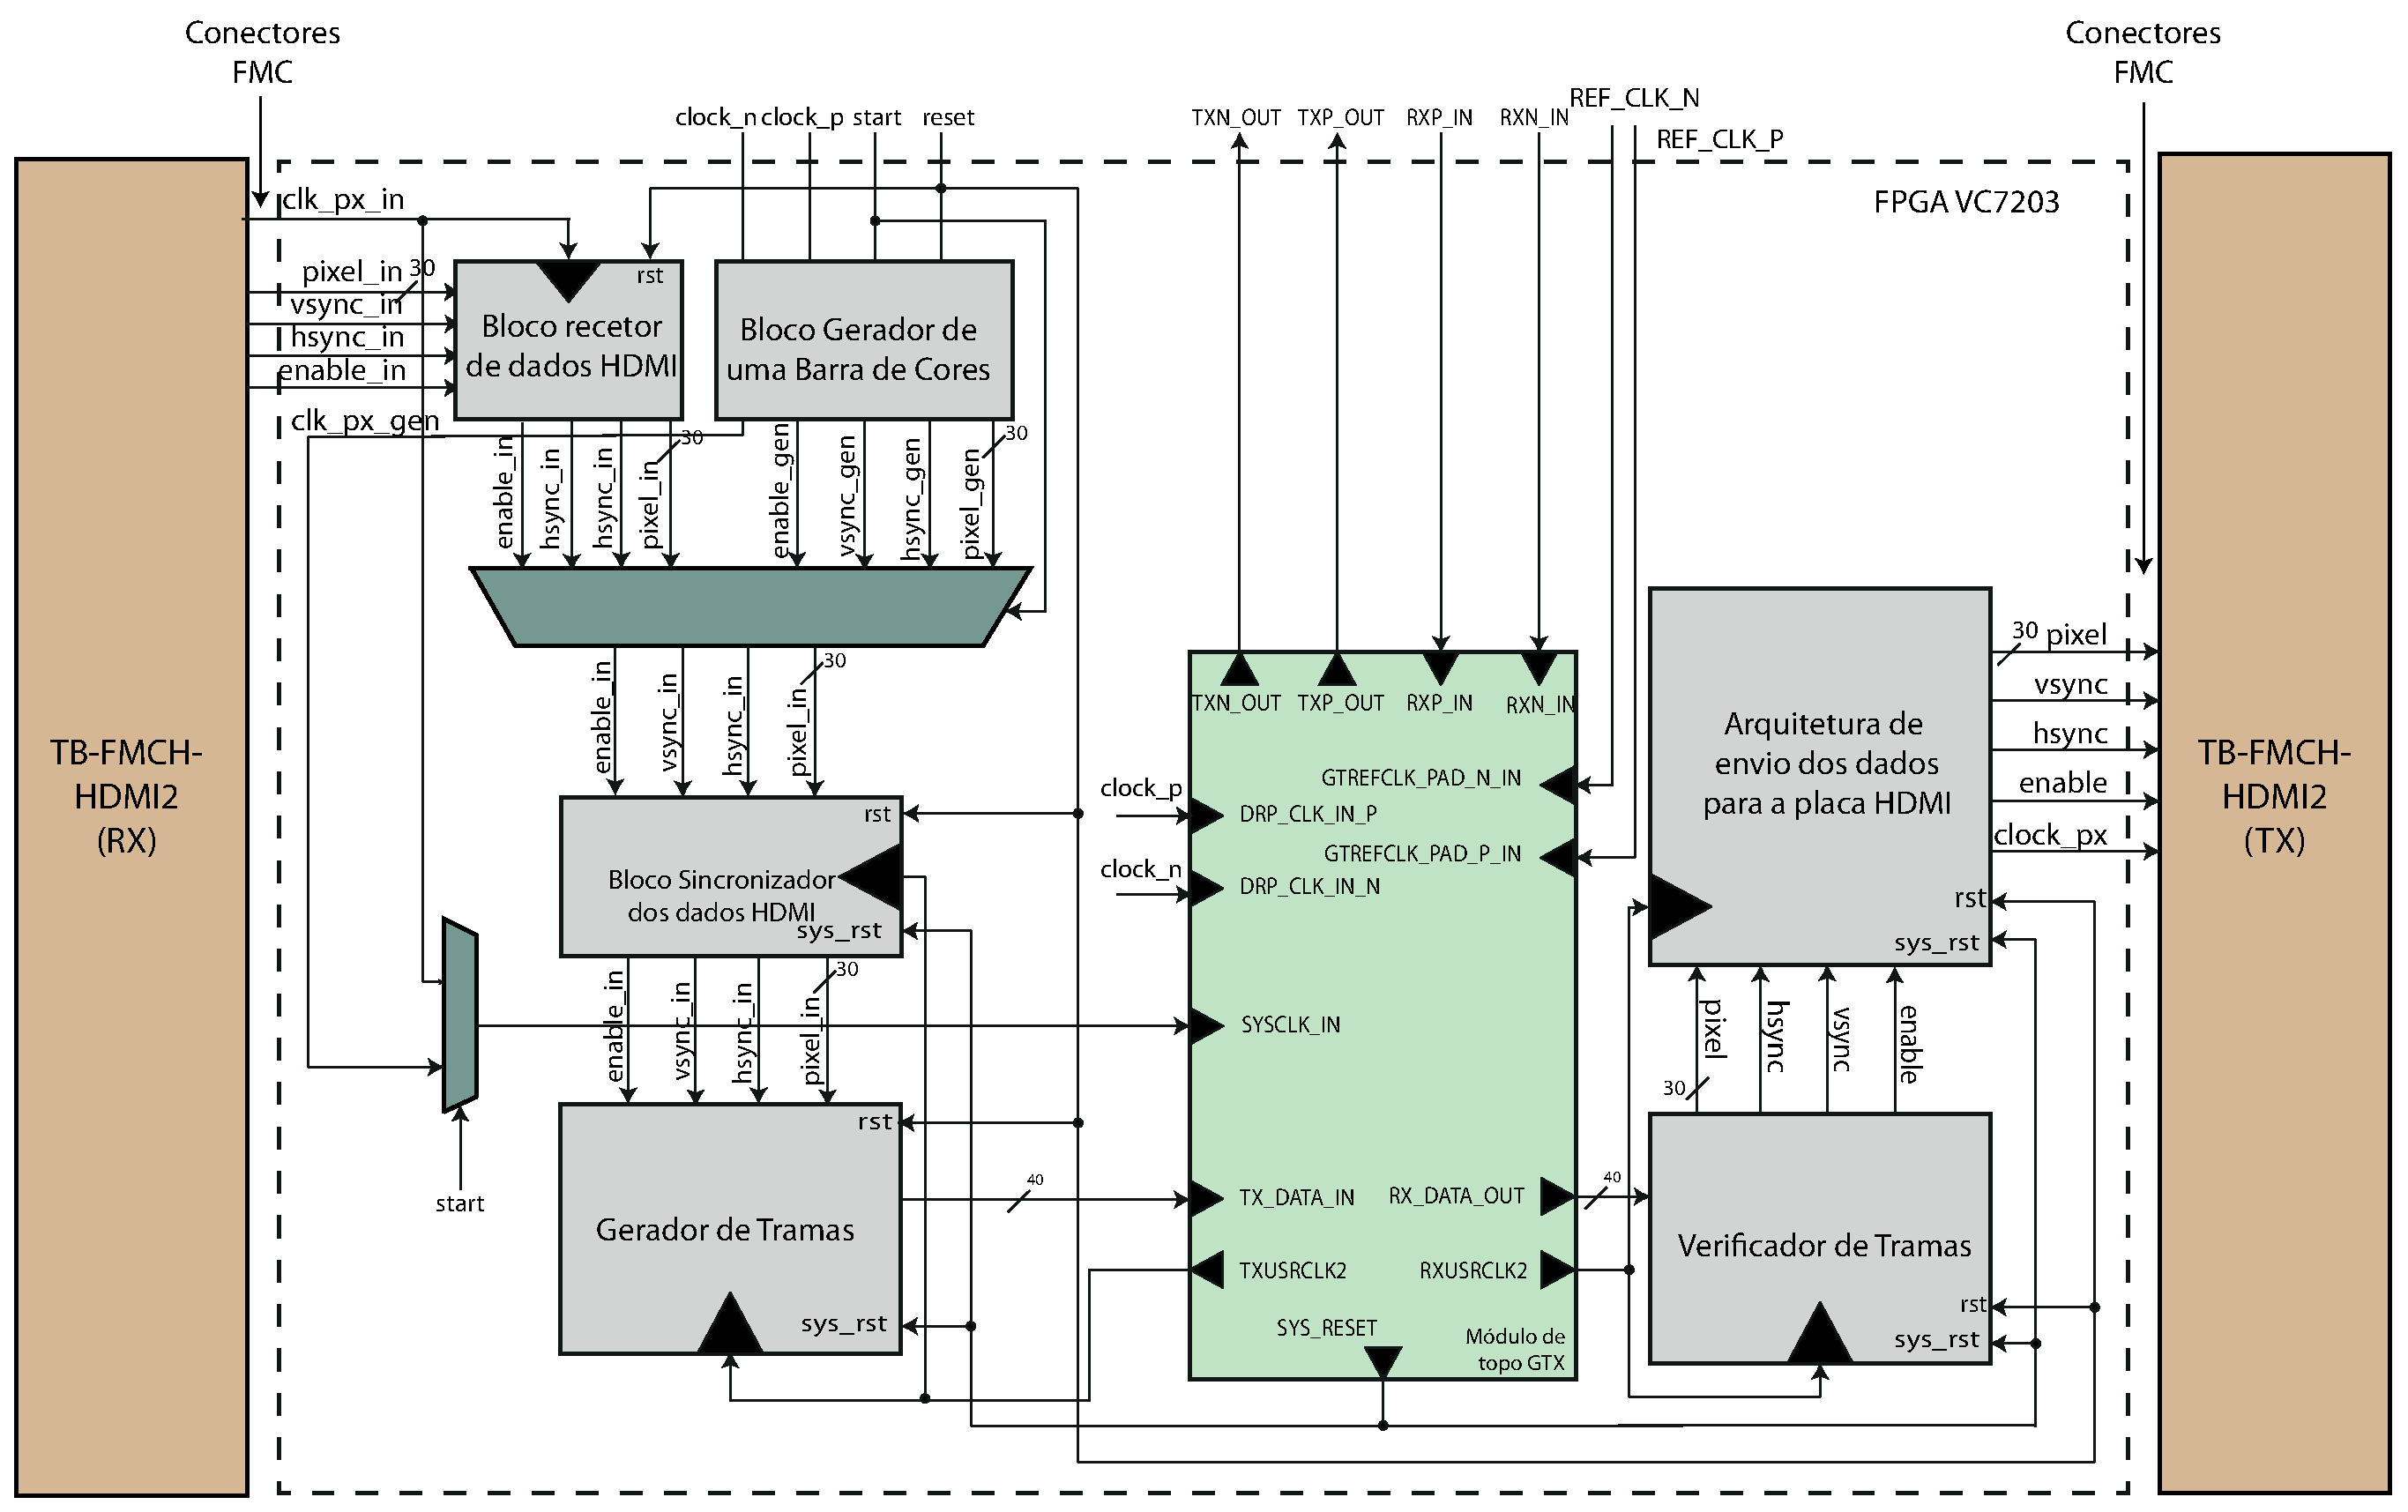
\includegraphics[width=1.0\textwidth]{planoE} 
			\caption{Diagrama de blocos da arquitetura E}
			\label{fig:planoE}
		\end{center}
		\end{figure}

	\subsubsection*{Bloco Recetor de dados HDMI}
	%explicar o que faz
	O bloco recetor de dados HDMI recebe os dados provenientes da placa recetora e guarda-os em registos síncronos com o flanco positivo do sinal de relógio proveniente da mesma. O diagrama de blocos deste módulo visualiza-se na figura \ref{fig:recetorHDMI}.
	%explicar o porque de ser necessário
	\begin{figure}[h!]
		\begin{center}
			\leavevmode
			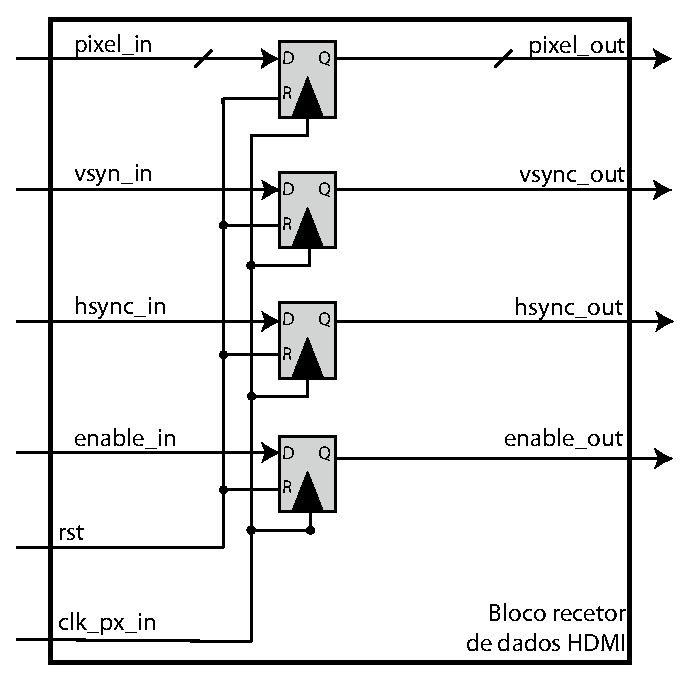
\includegraphics[width=0.5\textwidth]{recetorHDMI}
			\caption[Bloco recetor de dados HDMI]{Bloco Recetor de dados HDMI}
			\label{fig:recetorHDMI}
		\end{center}
	\end{figure}
	
	É de relembrar que existem dois domínios de relógio principais quando se faz a transmissão de dados entre a placa HDMI recetora para o transcetor GTX: o sinal de relógio proveniente da placa HDMI e o sinal de relógio proveniente do transcetor. Apesar de já existir um bloco responsável pela sincronização de dados do domínio do sinal de relógio TXUSRCLK2, o autor de \cite{R024} recomenda que também haja sincronização do lado do domínio que envia os dados. Apesar de as saídas da placa HDMI serem amostradas a uma determinada cadência, segundo os manuais das mesmas (\cite{R009}, \cite{R014} e \cite{R013}), pode existir algum desfasamento de dados que possa vir a provocar meta-estabilidade. Assim sendo, optou-se por criar este bloco.
	
	\subsubsection*{Localizações das portas de saída do módulo de topo} \label{subsub:serial_locs_planE}

	As localizações físicas das portas de entrada e saída do bloco encontram-se detalhadas na tabela \ref{table:LOC_simples_planE}. Como se pode observar, existem algumas portas que não estão representadas na figura \label{fig:planE} para simplificá-la. Essas portas são provenientes do módulo verificador de tramas e a sua principal função é manter o utilizador a par dos estados da transmissão do lado do recetor.  As mesmas são referidas na tabela com os nomes de ``\textit{begin\_state}'', ``\textit{SOP\_detected}'', ``\textit{track\_data}'', ``\textit{data\_error\_detected }'', ``\textit{idle\_slip}'', ``\textit{wait\_state}'' e ``\textit{align}'' e correspondem aos diferentes estados da máquina apresentada na secção \ref{subsub:serial_frameChecker} na página \pageref{subsub:serial_frameChecker}.
	
	A seleção dos dados no multiplexador que se visualiza na figura \ref{fig:planoE} é feita de acordo com o interruptor \textit{start} controlado pelo utilizador.
	
	\begin{table}[h!]
		\centering
		\caption{Localizações físicas das portas de entrada e saída da arquitetura}
		\label{table:LOC_simples_planE}
		\begin{tabular}{rlll}
			\hline
			\multicolumn{1}{l}{}                  & \multicolumn{1}{c}{\textbf{Sinal}}     & \multicolumn{1}{c}{\textbf{LOC na FPGA}} & \multicolumn{1}{c}{\textbf{Banco na FPGA}} \\ \hline
			\multicolumn{1}{r|}{\textbf{Entrada}} & clk\_p                                 & E19                                      & 38                                         \\
			\multicolumn{1}{r|}{\textbf{Entrada}} & clk\_n                                 & E18                                      & 38                                         \\
			\multicolumn{1}{r|}{\textbf{Entrada}} & reset                                  & N41                                      & 19                                         \\
			\multicolumn{1}{r|}{\textbf{Entrada}} & start                                  & E42                                      & 19                                         \\
			\multicolumn{1}{r|}{\textbf{Entrada}} & REF\_CLK\_P                            & AF8                                      & 114                                        \\
			\multicolumn{1}{r|}{\textbf{Entrada}} & REF\_CLK\_N                            & AF7                                      & 114                                        \\
			\multicolumn{1}{r|}{\textbf{Entrada}} & RXP\_IN                                & AG6                                      & 114                                        \\
			\multicolumn{1}{r|}{\textbf{Entrada}} & RXN\_IN                                & AG5                                      & 114                                        \\
			\multicolumn{1}{r|}{\textbf{Entrada}} & clk\_px\_in                            & AJ32                                     & 14                                         \\
			\multicolumn{1}{r|}{\textbf{Entrada}} & enable\_in                             & AN38                                     & 15                                         \\
			\multicolumn{1}{r|}{\textbf{Entrada}} & hsync\_in                              & AU39                                     & 15                                         \\
			\multicolumn{1}{r|}{\textbf{Entrada}} & vsync\_in                              & AU38                                     & 15                                         \\
			\multicolumn{1}{r|}{\textbf{Entrada}} & pixel\_in {[}0{]} a pixel\_in {[}29{]} & Ver \cite{R041}                                & 14 e 15                                    \\
			\multicolumn{1}{r|}{\textbf{Saída}}   & TXN\_OUT                               & AK3                                      & 114                                        \\
			\multicolumn{1}{r|}{\textbf{Saída}}   & TXP\_OUT                               & AK4                                      & 114                                        \\
			\multicolumn{1}{r|}{\textbf{Saída}}   & begin\_state                           & M38                                      & 19                                         \\
			\multicolumn{1}{r|}{\textbf{Saída}}   & SOP\_detected                          & R42                                      & 19                                         \\
			\multicolumn{1}{r|}{\textbf{Saída}}   & track\_data                            & P42                                      & 19                                         \\
			\multicolumn{1}{r|}{\textbf{Saída}}   & data\_error\_detected                  & N38                                      & 19                                         \\
			\multicolumn{1}{r|}{\textbf{Saída}}   & idle\_slip                             & M39                                      & 19                                         \\
			\multicolumn{1}{r|}{\textbf{Saída}}   & wait\_state                            & R40                                      & 19                                         \\
			\multicolumn{1}{r|}{\textbf{Saída}}   & align                                  & P40                                      & 19                                         \\
			\multicolumn{1}{r|}{\textbf{Saída}}   & clk\_px                                & E34                                      & 35                                         \\
			\multicolumn{1}{r|}{\textbf{Saída}}   & enable                                 & K35                                      & 34                                         \\
			\multicolumn{1}{r|}{\textbf{Saída}}   & hsync                                  & M32                                      & 34                                         \\
			\multicolumn{1}{r|}{\textbf{Saída}}   & vsync                                  & L31                                      & 34                                         \\
			\multicolumn{1}{r|}{\textbf{Saída}}   & pixel{[}0{]} a pixel {[}29{]}          & Ver \cite{R041}                                & 34 e 35                                    \\ \hline
		\end{tabular}
	\end{table}
	

	\section{Configuração do \textit{setup}}
	
	\subsection{FPGA VC7203}
	
	A placa FPGA \textit{Virtex-7} deve ser programada com o \textit{bitstream} gerado pós-implementação da arquitetura no \textit{software} VIVADO, e deve ainda ser programado o módulo que gera o sinal de relógio de referência do GTX com o nome ``\textit{SuperClock2}''. É necessário ter em conta que a programação do módulo  ``\textit{SuperClock2}'' deve ser realizada em primeiro lugar.
	
	\subsubsection{Programação do módulo gerador do sinal de relógio de referência}

	\begin{itemize}
		\item A FPGA deve estar devidamente conectada ao computador através da porta USB;
		\item Após inicializado, deve ser escolhida a opção ``\textit{Open Hardware Manager}'' no VIVADO;
		\item De seguida deve ser escolhida a opção ``\textit{Open New Target}'' dentro de ``\textit{Open Target}'';
		\item Na nova janela aberta deve-se seleccionar a FPGA \textbf{XC7VX485T-3} e terminar até a janela fechar;
		\item De seguida, selecciona-se com o botão do lado direito do rato o componente \textbf{XC7VX485T-3}, escolhendo-se a opção ``\textit{Program Device}'';
		\item Nessa janela é seleccionado o bitstream que tem o nome ``\textit{top\_scm2.bit}'' na pasta `\textit{finalFolder/SuperClock2\_Programming}'';
		\item Por fim, em "\textit{Options}" deve ser selecionada a opção "\textit{Run Tcl Script}", escolhendo-se o ficheiro com o nome ``\textit{setup\_scm2\_148\_4.tcl}'' na pasta `\textit{finalFolder/SuperClock2\_Programming/CRIAR\_relogio}''; 
	\end{itemize}
	
	\subsubsection{Programação da FPGA com o respetivo \textit{bitstream}}
	
	\begin{itemize}
		\item A FPGA deve estar devidamente conectada ao computador através da porta USB;
		\item Após inicializado, deve ser escolhida a opção ``\textit{Open Hardware Manager}'' no VIVADO;
		\item De seguida deve ser escolhida a opção ``\textit{Open New Target}'' dentro de ``\textit{Open Target}'';
		\item Na nova janela aberta deve-se seleccionar a FPGA \textbf{XC7VX485T-3} e terminar até a janela fechar;
		\item De seguida, selecciona-se com o botão do lado direito do rato o componente \textbf{XC7VX485T-3}, escolhendo-se a opção ``\textit{Program Device}'';
		\item Nessa janela é seleccionado o \textit{bitstream} correspondente para cada arquitetura.
	\end{itemize}
	
	Mais informações sobre o \textit{software} VIVADO pode ser encontrado em \cite{R019}.
	
	\subsection{TB-FMCH-HDMI TX e TB-FMCH-HDMI RX}
	Estas placas devem estar configuradas por omissão para ambas as configurações. Para tal deve-se recorrer ao \textit{software iMPACT} e ainda ao programador JTAG (tal como indicado em \cite{R025}). Para cada uma das placas deve ser realizado o seguinte procedimento caso estas estejam programadas com outra configuração:
	
	\begin{itemize}
		\item O programador deve estar devidamente conectado à placa HDMI e ao computador;
		\item O \textit{software iMPACT} deve ser inicializado;
		\item Com o botão do lado direito do rato deve ser escolhida a opção ``Inicializar cadeia'';
		\item A PROM (\textit{Programmable read-only memory}) cujos detalhes podem ser encontrados em \cite{R026} da placa transmissora deve ser programada com o ficheiro com o nome ``\textit{tx\_fpga\_top.mcs}'' ou ``\textit{rx\_fpga\_top.mcs}'' que se encontram na pasta  ``\textit{finalFolder/HDMI\_programming/default}''.
	\end{itemize}
	
	\subsection{Arquitetura D}
		Na figura \ref{fig:setupD} está representado o \textit{setup} de teste para a arquitetura D. O \textit{bitstream} correspondente a esta configuração tem o nome de ``\textit{gtwizard\_0\_exdes.bit}'' e encontra-se na pasta ``\textit{finalFolder/planD}''.
			\begin{figure}[h!]
			\begin{center}
				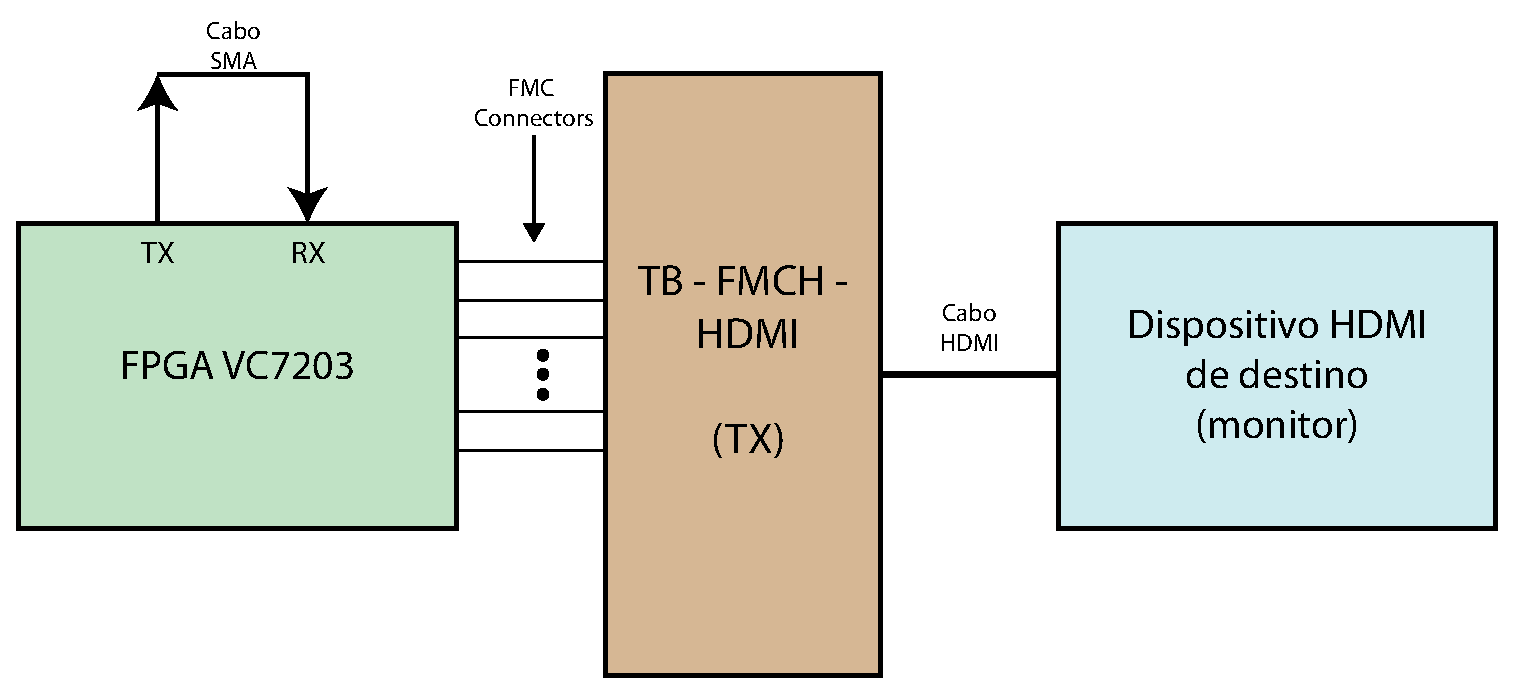
\includegraphics[width=1.0\textwidth]{planDsch} 
				\caption{\textit{Setup} de teste da arquitetura D}
				\label{fig:setupD}
			\end{center}
		\end{figure}
	\subsection{Arquitetura E}
		Na figura \ref{fig:setupE} está representado o \textit{setup} de teste para a arquitetura E. O \textit{bitstream} correspondente a esta configuração tem o nome de ``\textit{gtwizard\_0\_exdes.bit}'' e encontra-se na pasta ``\textit{finalFolder/planE}''.
		
		\begin{figure}[h!]
		\begin{center}
			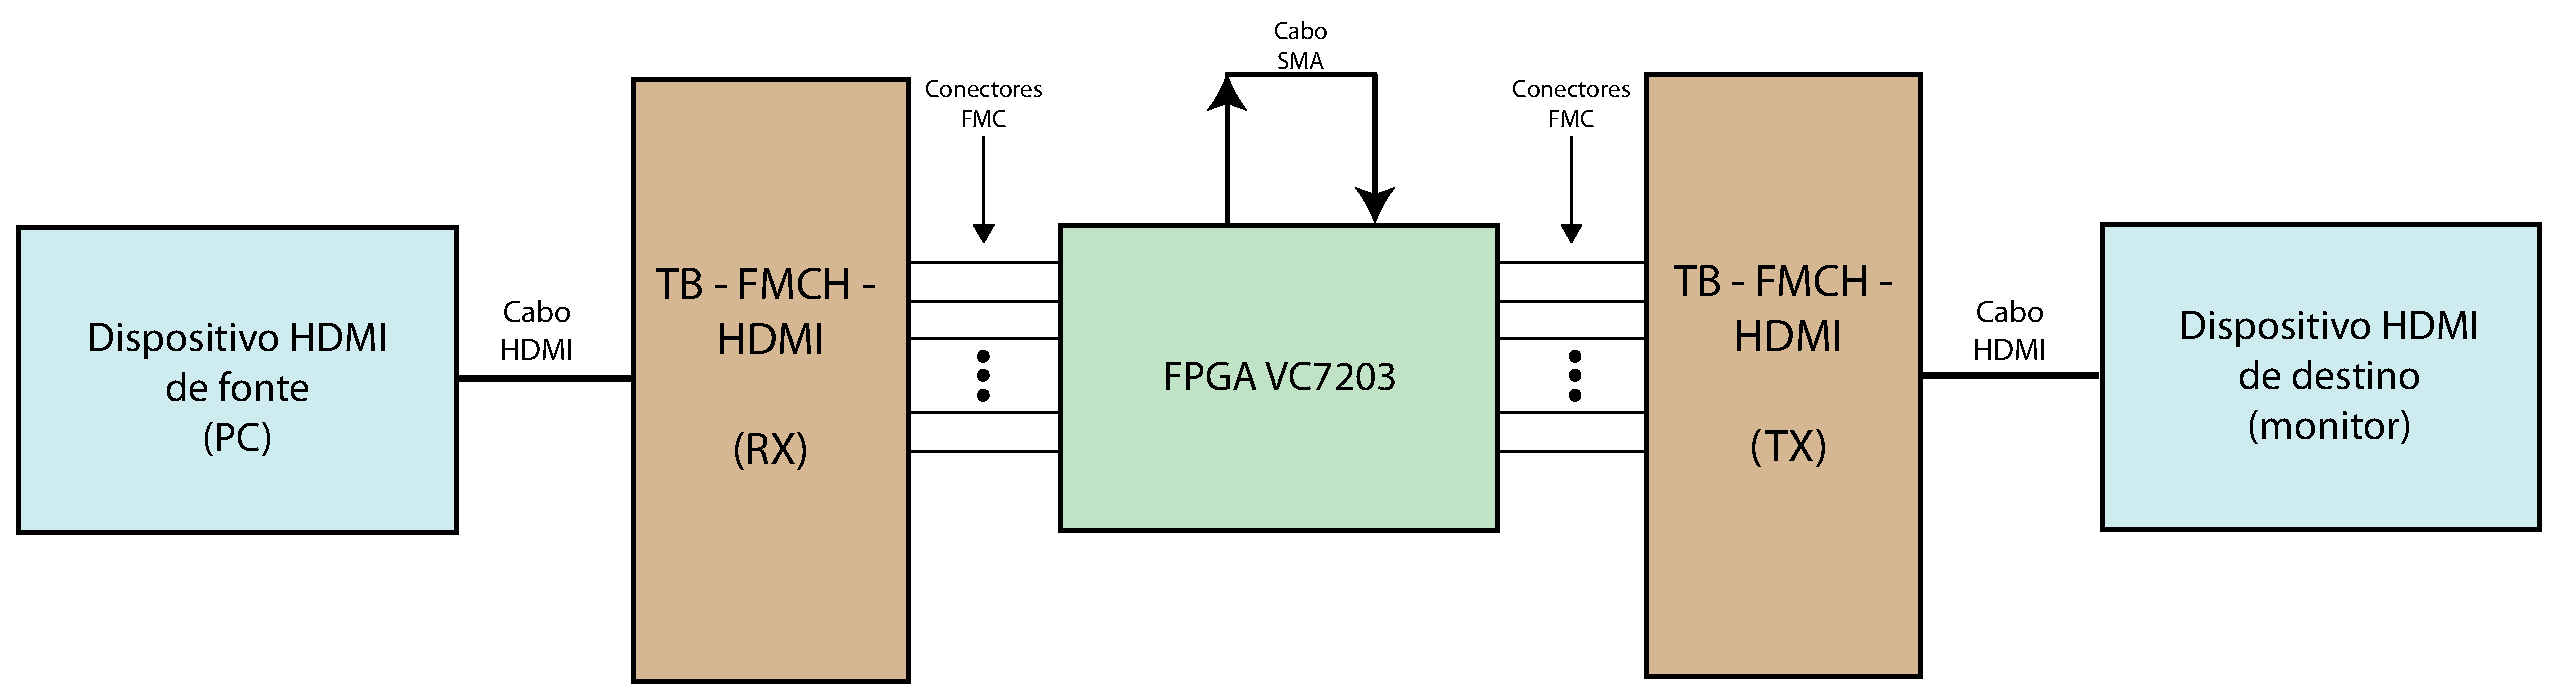
\includegraphics[width=1.0\textwidth]{planEsch} 
			\caption{\textit{Setup} de teste da arquitetura E}
			\label{fig:setupE}
		\end{center}
	\end{figure}



	\section{Utilização dos recursos da FPGA}
	
	Na Tabela \ref{table:recursos_planoD_planoE} são apresentados os valores dos recursos utilizados pela FPGA nestas arquiteturas.

\begin{table}[h!]
	\centering
	\caption{Recursos utilizados pelas arquiteturas desenvolvidas de transmissão em série}
	\label{table:recursos_planoD_planoE}
	
	\begin{tabular}{rllll}
		\hline
		\multicolumn{1}{c}{\multirow{2}{*}{\textbf{Recurso}}} & \multicolumn{2}{c}{\textbf{Arquitetura D}}                                 & \multicolumn{2}{c}{\textbf{Arquitetura E}}                               \\ \cline{2-5} 
		\multicolumn{1}{c}{}                                  & \multicolumn{1}{c}{\textbf{Utilização}} & \multicolumn{1}{c|}{\textbf{\%}} & \multicolumn{1}{c}{\textbf{Utilização}} & \multicolumn{1}{c}{\textbf{\%}} \\ \hline
		\multicolumn{1}{r|}{\textbf{FF}}                      & 566                                     & \multicolumn{1}{l|}{0,09}        & 710                                    & 0,12                            \\
		\multicolumn{1}{r|}{\textbf{LUT}}                     & 486                                     & \multicolumn{1}{l|}{0,16}        & 590                                    & 0,19                            \\
		\multicolumn{1}{r|}{\textbf{I/O}}                     & 44                                      & \multicolumn{1}{l|}{6,29}        & 78                                     & 11,14                           \\
		\multicolumn{1}{r|}{\textbf{GT}}                      & 1                                       & \multicolumn{1}{l|}{2,86}        & 1                                      & 2,86                            \\ \hline
	\end{tabular}%
\end{table}
	
	Os valores percentuais ocupados pelas arquiteturas são muito baixos, possibilitando a expansão das mesmas caso necessário. 
	
	
	\section{Resultados}
	\subsection{Arquitetura D}

	Os resultados obtidos foram os esperados: a transmissão em série foi bem sucedida e visualizou-se uma barra de cores no monitor, tal como se visualiza na figura \ref{fig:planD_resultados}. Para além disto, quando se desconectam os conectores SMA, a ligação perde-se e quando se voltam a conectar, a mesma é recuperada, o que vem validar a máquina de estados desenvolvida.

	
	\begin{figure}[h!]
		\begin{center}
			\leavevmode
			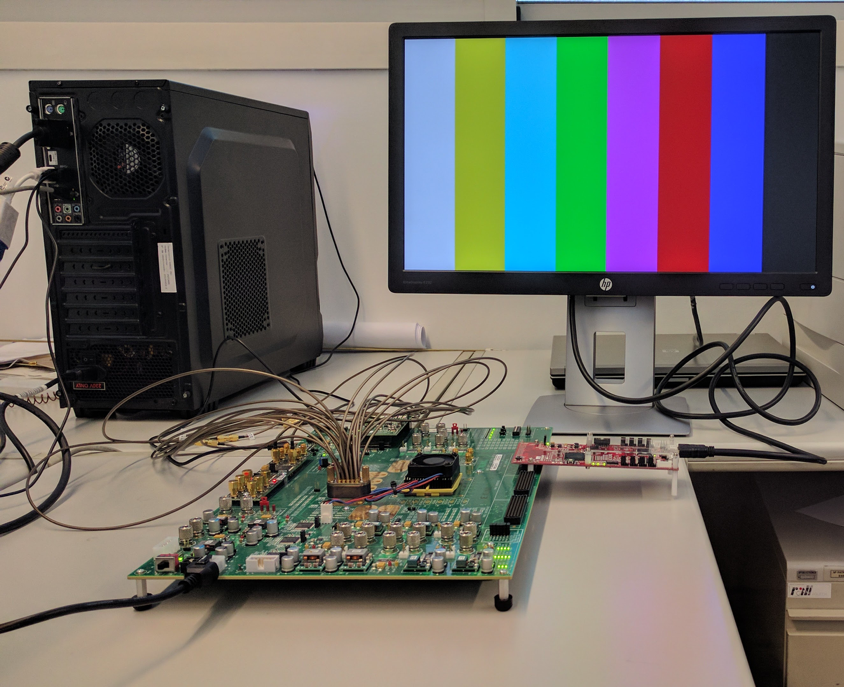
\includegraphics[width=0.7\textwidth]{resultados_planoD}
			\caption[Resultados obtidos da transmissão em série de uma barra de cores gerada na FPGA]{Resultados obtidos da transmissão em série de uma barra de cores gerada na FPGA}
			\label{fig:planD_resultados}
		\end{center}
	\end{figure}
	\subsection{Arquitetura E}
	
	Obteve-se uma transmissão em série como pretendido entre ambos os dispositivos, mas surgiu um problema. Apesar de nas diversas simulações realizadas (funcional, pós-síntese e pós-implementação) a arquitetura ter sido validada, quando se implementa a mesma na FPGA ocorre um problema de visualização da imagem no dispositivo de destino: são apresentadas umas ligeiras riscas pretas horizontais. O resultado está apresentado na figura \ref{fig:planoE_results}.
	
	
	\begin{figure}
		\begin{center}
			\leavevmode
			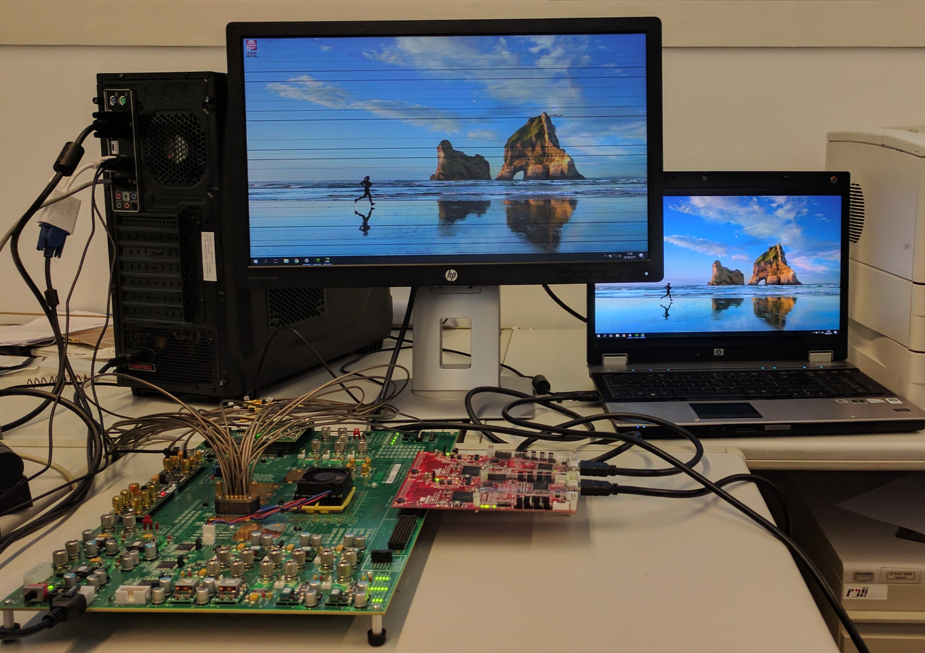
\includegraphics[width=0.7\textwidth]{resultados_planoE}		
			\caption[Resultado obtido da arquitetura de transmissão em série entre dispositivos HDMI]{Resultado obtido da arquitetura de transmissão em série entre dispositivos HDMI}
			\label{fig:planoE_results}
		\end{center}
	\end{figure}
	
	%explicar problema
	O problema foi diagnosticado recorrendo-se à utilização de um \textit{IP} da Xilinx, designado por ILA (\textit{Integrated Logic Analyzer}), que permite monitorizar os sinais internos da FPGA através das suas diversas características tendo como base de tempo o sinal de relógio de referência do mesmo. O problema não se deve à transmissão em série, mas sim a uma falha sincronização entre registos antes de se realizar a mesma.
	
	\begin{figure}
		\begin{center}
			\leavevmode
			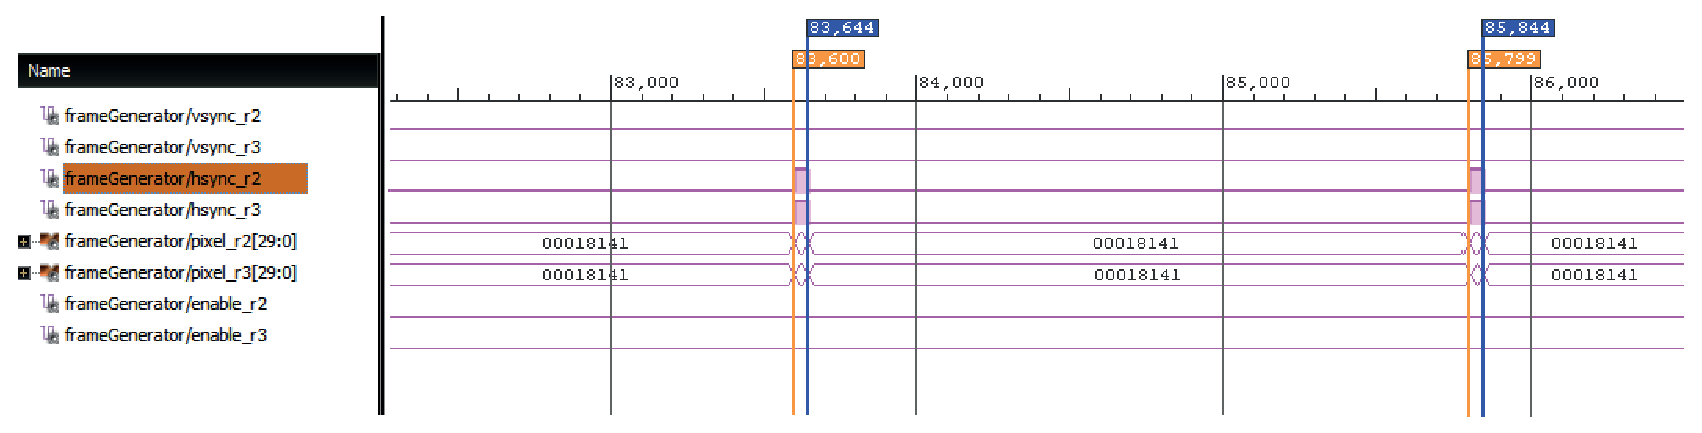
\includegraphics[width=1.0\textwidth]{erro_planoE}
			\caption[Gráfico da análise do comportamento dos sinais internos da FPGA]{Gráfico da análise do comportamento dos sinais internos da FPGA}
			\label{fig:planoE_rerro}
		\end{center}
	\end{figure}
	
	Na figura \ref{fig:planoE_rerro} é possível visualizar um gráfico retirado da análise dos sinais internos da FPGA. De notar que a base de tempo é o sinal de relógio de referência, que para este caso foi TXUSRCLK2 (proveniente do GTX), e por isso uma unidade na figura representa um ciclo de relógio do mesmo.  Neste gráfico estão a ser analisadas as transições dos dados do sub-módulo do sistema ``Bloco Recetor de dados HDMI'' para o ``Bloco Sincronizador dos dados HDMI''. Os sinais ``\textit{hsync\_r2}'' e ``\textit{hsync\_r3}'' no gráfico correspondem aos dois registos de sincronização do bloco ``Sincronizador dos dados HDMI'' ilustrado na figura \ref{fig:sync_block}.
	
	O que está a causar o problema, através da análise feita, é a falha num ciclo de relógio de uma linha inteira. Ou seja, na primeira transição que se vê no sinal \textit{hsync\_r2} o seu comportamento é como esperado: tem um tempo de duração de 44 ciclos de relógio e encontra-se no início da transmissão de uma linha completa. No entanto, na segunda transição do mesmo o seu comportamento não é o esperado: tem um tempo de duração de 45 ciclos de relógio e fica ativo um ciclo de relógio antes do início da linha. Relembrando que uma linha completa tem 2200 ciclos de relógio, a diferença entre a primeira transição de 0 para 1 do sinal em questão para a segunda é de 2199 ciclos de relógio. 
	
	Este problema acaba por acontecer em várias linhas causando uma falha na sincronização horizontal da imagem, o que provoca as ligeiras riscas pretas que se visualizam na imagem recebida.
	
	%explicar como soluccionar o problema
	
	Assim, conclui-se que apesar da transmissão em série estar a operar como esperado, o processo de transmissão de dados não é robusto. Os sinais são transmitidos diretamente e apesar de ter havido precauções quanto ao sincronismo entre os domínios de relógio, existiu uma falha de sincronismo.
	%-------------------------------------------------------------------------
	%	BIBLIOGRAPHY
	%----------------------------------------------------------------------------------------
	
	\bibliographystyle{ieeetr}
	
	\bibliography{myrefs}
	
	
	%----------------------------------------------------------------------------------------
%	\begin{table}[h!]
%		\centering
%		\caption{Recursos utilizados pelas diferentes arquiteturas implementadas na FPGA}
%		\label{table:recursos_a_b_c}
%		\resizebox{\textwidth}{!}{%
%			\begin{tabular}{l|ll|ll|ll}
%				\hline
%				\multicolumn{1}{c|}{\multirow{2}{*}{\textbf{Recurso}}} & \multicolumn{2}{r|}{\textbf{Arquitetura A}}                                 & \multicolumn{2}{r|}{\textbf{Arquitetura B}}                                & \multicolumn{2}{r}{\textbf{Arquitetura C}}                               \\ \cline{2-7} 
%				\multicolumn{1}{c|}{}                                  & \multicolumn{1}{c}{\textbf{Utilização}} & \multicolumn{1}{c|}{\textbf{\%}} & \multicolumn{1}{c}{\textbf{Utilização}} & \multicolumn{1}{c|}{\textbf{\%}} & \multicolumn{1}{c}{\textbf{Utilização}} & \multicolumn{1}{c}{\textbf{\%}} \\ \hline
%				\textbf{FF}                                            & 31                                      & 0,01                             & 64                                      & 0,01                            & 59                                      & 0,01                            \\
%				\textbf{LUT}                                           & 59                                      & 0,02                             & 67                                      & 0,02                            & 27                                      & 0,01                            \\
%				\textbf{I/O}                                           & 38                                      & 5,43                             & 70                                      & 10                               & 103                                     & 14,71                           \\
%				\textbf{GT}                                            & 0                                       & 0                                & 0                                       & 0                                & 0                                       & 0                               \\ \hline
%			\end{tabular}%
%		}
%	\end{table}
%
%\begin{table}[h!]
%	\centering
%	\caption{Recursos utilizados pelas arquiteturas desenvolvidas de transmissão em série}
%	\label{table:recursos_planoD_planoE}
%	
%	\begin{tabular}{rllll}
%		\hline
%		\multicolumn{1}{c}{\multirow{2}{*}{\textbf{Recurso}}} & \multicolumn{2}{c}{\textbf{Arquitetura D}}                                 & \multicolumn{2}{c}{\textbf{Arquitetura E}}                               \\ \cline{2-5} 
%		\multicolumn{1}{c}{}                                  & \multicolumn{1}{c}{\textbf{Utilização}} & \multicolumn{1}{c|}{\textbf{\%}} & \multicolumn{1}{c}{\textbf{Utilização}} & \multicolumn{1}{c}{\textbf{\%}} \\ \hline
%		\multicolumn{1}{r|}{\textbf{FF}}                      & 566                                     & \multicolumn{1}{l|}{0,09}        & 710                                    & 0,12                            \\
%		\multicolumn{1}{r|}{\textbf{LUT}}                     & 486                                     & \multicolumn{1}{l|}{0,16}        & 590                                    & 0,19                            \\
%		\multicolumn{1}{r|}{\textbf{I/O}}                     & 44                                      & \multicolumn{1}{l|}{6,29}        & 78                                     & 11,14                           \\
%		\multicolumn{1}{r|}{\textbf{GT}}                      & 1                                       & \multicolumn{1}{l|}{2,86}        & 1                                      & 2,86                            \\ \hline
%	\end{tabular}%
%\end{table}

	
\end{document}